%% abtex2-modelo-artigo.tex, v-1.9.7 laurocesar
%% Copyright 2012-2018 by abnTeX2 group at http://www.abntex.net.br/ 
%%
%% This work may be distributed and/or modified under the
%% conditions of the LaTeX Project Public License, either version 1.3
%% of this license or (at your option) any later version.
%% The latest version of this license is in
%%   http://www.latex-project.org/lppl.txt
%% and version 1.3 or later is part of all distributions of LaTeX
%% version 2005/12/01 or later.
%%
%% This work has the LPPL maintenance status `maintained'.
%% 
%% The Current Maintainer of this work is the abnTeX2 team, led
%% by Lauro César Araujo. Further information are available on 
%% http://www.abntex.net.br/
%%
%% This work consists of the files abntex2-modelo-artigo.tex and
%% abntex2-modelo-references.bib
%%

% ------------------------------------------------------------------------
% ------------------------------------------------------------------------
% abnTeX2: Modelo de Artigo Acadêmico em conformidade com
% ABNT NBR 6022:2018: Informação e documentação - Artigo em publicação 
% periódica científica - Apresentação
% ------------------------------------------------------------------------
% ------------------------------------------------------------------------

\documentclass[
	% -- opções da classe memoir --
	article,			% indica que é um artigo acadêmico
	11pt,				% tamanho da fonte
	oneside,			% para impressão apenas no recto. Oposto a twoside
	a4paper,			% tamanho do papel. 
	% -- opções da classe abntex2 --
	%chapter=TITLE,		% títulos de capítulos convertidos em letras maiúsculas
	%section=TITLE,		% títulos de seções convertidos em letras maiúsculas
	%subsection=TITLE,	% títulos de subseções convertidos em letras maiúsculas
	%subsubsection=TITLE % títulos de subsubseções convertidos em letras maiúsculas
	% -- opções do pacote babel --
	english,			% idioma adicional para hifenização
	brazil,				% o último idioma é o principal do documento
	sumario=tradicional
	]{abntex2}


% ---
% PACOTES
% ---

% ---
% Pacotes fundamentais 
% ---
\usepackage[alf]{abntex2cite}
\usepackage{lmodern}			% Usa a fonte Latin Modern
\usepackage[T1]{fontenc}		% Selecao de codigos de fonte.
\usepackage[utf8]{inputenc}		% Codificacao do documento (conversão automática dos acentos)
\usepackage{indentfirst}		% Indenta o primeiro parágrafo de cada seção.
\usepackage{nomencl} 			% Lista de simbolos
\usepackage{color}				% Controle das cores
\usepackage{graphicx}			% Inclusão de gráficos
\usepackage{microtype} 			% para melhorias de justificação
\usepackage{svg}
\usepackage{subcaption}
\usepackage{amsmath}
\usepackage{tikz}
\usepackage{float}
% ---
		
% ---
% Pacotes adicionais, usados apenas no âmbito do Modelo Canônico do abnteX2
% ---
\usepackage{lipsum}				% para geração de dummy text
% ---
		
% ---
% Pacotes de citações
% ---
\usepackage[brazilian,hyperpageref]{backref}	 % Paginas com as citações na bibl
\usepackage[alf]{abntex2cite}	% Citações padrão ABNT
% ---

% ---
% Configurações do pacote backref
% Usado sem a opção hyperpageref de backref
\renewcommand{\backrefpagesname}{Citado na(s) página(s):~}
% Texto padrão antes do número das páginas
\renewcommand{\backref}{}
% Define os textos da citação
\renewcommand*{\backrefalt}[4]{
	\ifcase #1 %
		Nenhuma citação no texto.%
	\or
		Citado na página #2.%
	\else
		Citado #1 vezes nas páginas #2.%
	\fi}%
% ---

% --- Informações de dados para CAPA e FOLHA DE ROSTO ---
\titulo{Relatório - Projeto \\ Inteligência Artificial}
\tituloestrangeiro{Report - Project \\ Artificial Intelligence }

\autor{
Matheus H. Pimenta Z. \\\url{https://github.com/omatheuspimenta/IA_project} \thanks{matheus.pimenta@outlook.com}}

\local{Brasil}
\data{2021}
% ---

% ---
% Configurações de aparência do PDF final

% alterando o aspecto da cor azul
\definecolor{blue}{RGB}{41,5,195}

% informações do PDF
\makeatletter
\hypersetup{
     	%pagebackref=true,
		pdftitle={\@title}, 
		pdfauthor={\@author},
    	pdfsubject={Modelo de artigo científico com abnTeX2},
	    pdfcreator={LaTeX with abnTeX2},
		pdfkeywords={abnt}{latex}{abntex}{abntex2}{atigo científico}, 
		colorlinks=true,       		% false: boxed links; true: colored links
    	linkcolor=blue,          	% color of internal links
    	citecolor=blue,        		% color of links to bibliography
    	filecolor=magenta,      		% color of file links
		urlcolor=blue,
		bookmarksdepth=4
}
\makeatother
% --- 

% ---
% compila o indice
% ---
\makeindex
% ---

% ---
% Altera as margens padrões
% ---
\setlrmarginsandblock{3cm}{3cm}{*}
\setulmarginsandblock{3cm}{3cm}{*}
\checkandfixthelayout
% ---

% --- 
% Espaçamentos entre linhas e parágrafos 
% --- 

% O tamanho do parágrafo é dado por:
\setlength{\parindent}{1.3cm}

% Controle do espaçamento entre um parágrafo e outro:
\setlength{\parskip}{0.2cm}  % tente também \onelineskip

% Espaçamento simples
\SingleSpacing


% ----
% Início do documento
% ----
\begin{document}

% Seleciona o idioma do documento (conforme pacotes do babel)
%\selectlanguage{english}
\selectlanguage{brazil}

% Retira espaço extra obsoleto entre as frases.
\frenchspacing 

% ----------------------------------------------------------
% ELEMENTOS PRÉ-TEXTUAIS
% ----------------------------------------------------------

%---
%
% Se desejar escrever o artigo em duas colunas, descomente a linha abaixo
% e a linha com o texto ``FIM DE ARTIGO EM DUAS COLUNAS''.
% \twocolumn[    		% INICIO DE ARTIGO EM DUAS COLUNAS
%
%---

% página de titulo principal (obrigatório)
\maketitle


% titulo em outro idioma (opcional)



% % resumo em português
\begin{resumoumacoluna}
 Linguagem: Python $3.8.8$
 
 Bibliotecas:
 \begin{verbatim}
    pandas
    seaborn
    sklearn
    matplotlib.pyplot
    numpy
    xgboost
 \end{verbatim}

 URL: \url{https://github.com/omatheuspimenta/IA_project}
 
 Todos os códigos estão no link acima. Neste relatório são apresentados algumas partes dos códigos apenas.
 %\vspace{\onelineskip}
 
 %\noindent
 %\textbf{Palavras-chave}: latex. abntex. editoração de texto.
\end{resumoumacoluna}


% resumo em inglês
% \renewcommand{\resumoname}{Abstract}
% \begin{resumoumacoluna}
%  \begin{otherlanguage*}{english}
%    According to ABNT NBR 6022:2018, an abstract in foreign language is optional.
% 
%    \vspace{\onelineskip}
%  
%    \noindent
%    \textbf{Keywords}: latex. abntex.
%  \end{otherlanguage*}  
% \end{resumoumacoluna}

% ]  				% FIM DE ARTIGO EM DUAS COLUNAS
% ---

% \begin{center}\smaller
% \textbf{Data de submissão e aprovação}: elemento obrigatório. Indicar dia, mês e ano
% 
% \textbf{Identificação e disponibilidade}: elemento opcional. Pode ser indicado 
% o endereço eletrônico, DOI, suportes e outras informações relativas ao acesso.
% \end{center}

% ----------------------------------------------------------
% ELEMENTOS TEXTUAIS
% ----------------------------------------------------------
\textual

% ----------------------------------------------------------
% Introdução
% ----------------------------------------------------------
\section{Dataset}

O dataset utilizado é composto por $50$ colunas que representam medidas topológicas de grafos extraídas através de \textit{thresholds} e mais uma coluna representando os rótulos das classes. Foram consideradas $200$ observações\footnote{A não consideração de um maior número de amostras não afetou o objetivo de apresentar o comportamento de diversos classificadores.} ao todo, sendo $50$ observações para cada uma das $4$ classes de elementos considerados. 

\begin{verbatim}
 #file: preprocess.ipynb
 #Leitura do dataset
 df = pd.read_csv("dataframe.csv", 
                  index_col = 0)
 #Dimensão do dataset
 df.shape
\end{verbatim}


A escolha do dataset em análise é justificada por trabalhos já publicados utilizando datasets similares, isto é, utilizando medidas topológicas extraídas a partir de grafos \cite{Childs2009, Ito2018}.

As etapas de pré-processamento realizadas neste dataset são apresentadas a seguir, salienta-se que por tratar-se de um dataset contendo apenas valores numéricos  muitas etapas não foram necessárias para a preparação e tratamento dos dados, contudo em outros tipos de dados etapas como remoção de valores faltantes, verificação de variáveis qualitativas, transformação de dados e etapas de processamento de texto, por exemplo são necessárias \cite{garcia2015data}.

\begin{verbatim}
 #file: preprocess.ipynb
 #Verificando a classe de cada coluna do dataset
 df.dtypes
\end{verbatim}

O primeiro tratamento realizado no dataset foi a verificação e remoção de colunas nulas, após a remoção das colunas nulas do dataset o tamanho final foi de $34$ colunas de características e $1$ coluna dos rótulos. Nenhuma observação foi desconsiderada.

\begin{verbatim}
 #file: preprocess.ipynb
 #Removendo colunas nulas
 df = df.loc[:, (df != 0).any(axis=0)]
 #Dimensão do dataset
 df.shape
\end{verbatim}

Após a remoção das colunas com valores nulos, uma normalização dos dados foi realizada com o objetivo de que todos os valores do dataset pertençam ao intervalo $[0,1]$. A normalização realizada foi utilizando o valor máximo e mínimo de cada uma das observações em relação a característica, como apresentado pela equação \ref{eq:minmax}:

\begin{equation}
\label{eq:minmax}
 x_{scale} = \frac{x - \min_{C}{(x)}}{\max_{C}{(x)}-\min_{C}{(x)}},
\end{equation}
onde $x$ é o valor da observação, $\min_{C}{(x)}$ e $\max_{C}{(x)}$ são o valor mínimo e máximo da característica observada, respectivamente.

A normalização é utilizada para homogeneizar os dados, diminuir viéses existentes na geração dos dados e para reduzir efeitos de ``valorização'' de um dado em relação a outros devido a escala de cada característica. O pacote \verb|preprocessing| da biblioteca \verb|sklearn| foi utilizado para a normalização MinMax do dataset.

\begin{verbatim}
 #file: preprocess.ipynb
 #Normalização dos dados utilizando MinMax
 min_max_scaler = preprocessing.MinMaxScaler()
 df_minmax = min_max_scaler.fit_transform(df)
 df = pd.DataFrame(df_minmax)
\end{verbatim}


\subsection{Caracterização do Dataset}

Para as representações visuais do dataset foram consideradas apenas $10$ colunas, sendo a primeira coluna de cada uma das $10$ medidas topológicas consideradas.

Optou-se considerar apenas $10$ colunas devido a limitação computacional da execução de um número maior de colunas, além da poluição visual caso sejam consideradas todas as $50$ colunas.

A representação utilizando gráficos do tipo \textit{scatter plot} são apresentadas nas figuras \ref{fig:scatter_hist01}, \ref{fig:scatter_hist02}, \ref{fig:scatter_kde01} e \ref{fig:scatter_kde02}. Nas diagonais estão representados os histogramas das características e a distribuição de densidade, respectivamente. A distribuição de densidade das variáveis é uma maneira de visualizar o comportamento da variável contínua nas observações, o que é recomendado já que o dataset é composto por variáveis contínuas.

A dispersão dos pontos, indicam que entre algumas características existe correlação já que a disposição assemelha-se a uma reta, como é o caso das características MT4 e MT3, o que de fato é coerente visto que MT3 está relacionado ao número de motifs com $3$ vértices e MT4 relaciona-se com motifs de tamanho $4$. Além da análise de correlação, a caracterização das frequências no histograma pode levantar hipóteses em relação a natureza das características, como por exemplo assumir a normalidade de algumas variáveis, como é o caso da característica ASS.

\begin{verbatim}
 #file: preprocess.ipynb
 #Scatter plot com histogramas
 pd.plotting.scatter_matrix(df[['ASS.1', 'BET.1', 'ASPL.1', 'CC.1', 'DEG.1',
 'MIN.1', 'MAX.1',  'SD.1', 'MT3.1', 'MT4.1']], figsize=(10,10))
 
 #Scatter plot com distribuição de densidade
 pd.plotting.scatter_matrix(df[['ASS.1', 'BET.1', 'ASPL.1', 'CC.1', 'DEG.1',
 'MIN.1', 'MAX.1',  'SD.1', 'MT3.1', 'MT4.1']], diagonal = 'kde',
 figsize=(10,10))
\end{verbatim}

Além das representações e gráficos \textit{scatter plot}, foram extraídas informações estatísticas do dataset em análise. Os dados são apresentados nas tabelas \ref{tab:est_ori} e \ref{tab:est_norm}.

\begin{verbatim}
 #file: preprocess.ipynb
 #Medidas de posição e dispersão do dataset
 pd.options.display.float_format = "{:.3f}".format
 df.describe().T
\end{verbatim}


Após a normalização, um \textit{boxplot} e um \textit{violin plot} foram utilizados para a visualização da distribuição dos dados dentro do intervalo $[0,1]$, como apresentado nas figuras \ref{fig:boxplot} e \ref{fig:violin}. A escolha do \textit{violin plot} é justificada pela alta frequência de valores considerados outliers nas amostras, como apresentado pelo \textit{boxplot}, dessa maneira é possível verificar em qual região do intervalo está a maior concentração dos dados.

\begin{verbatim}
 #file: preprocess.ipynb
 #Boxplot
 boxplot = df.boxplot(column=['ASS.1', 'BET.1', 'ASPL.1', 'CC.1', 'DEG.1',
 'MIN.1', 'MAX.1',  'SD.1', 'MT3.1', 'MT4.1'], figsize=(10,8))
 
 #Violin plot
 fig, axes = plt.subplots(figsize=(10,8))
 labels = ['ASS.1', 'BET.1', 'ASPL.1', 'CC.1', 'DEG.1', 'MIN.1',
 'MAX.1',  'SD.1', 'MT3.1', 'MT4.1']

 axes.violinplot(dataset=[df["ASS.1"],
                          df["BET.1"],
                          df["ASPL.1"],
                          df["CC.1"],
                          df["DEG.1"],
                          df["MIN.1"],
                          df["MIN.1"],
                          df["MAX.1"],
                          df["SD.1"],
                          df["MT3.1"],
                          df["MT4.1"]])
 axes.set_title('Dataset Overview')
 axes.yaxis.grid(True)
 axes.set_ylabel('Values')
 axes.xaxis.set_tick_params(direction='out')
 axes.xaxis.set_ticks_position('bottom')
 axes.set_xticks(np.arange(1, len(labels) + 1))
 axes.set_xticklabels(labels)
 axes.set_xlim(0.25, len(labels) + 0.75)
 axes.set_xlabel('Features names')
 plt.show()
\end{verbatim}

\newpage
\begin{figure}[H]
 \centering
 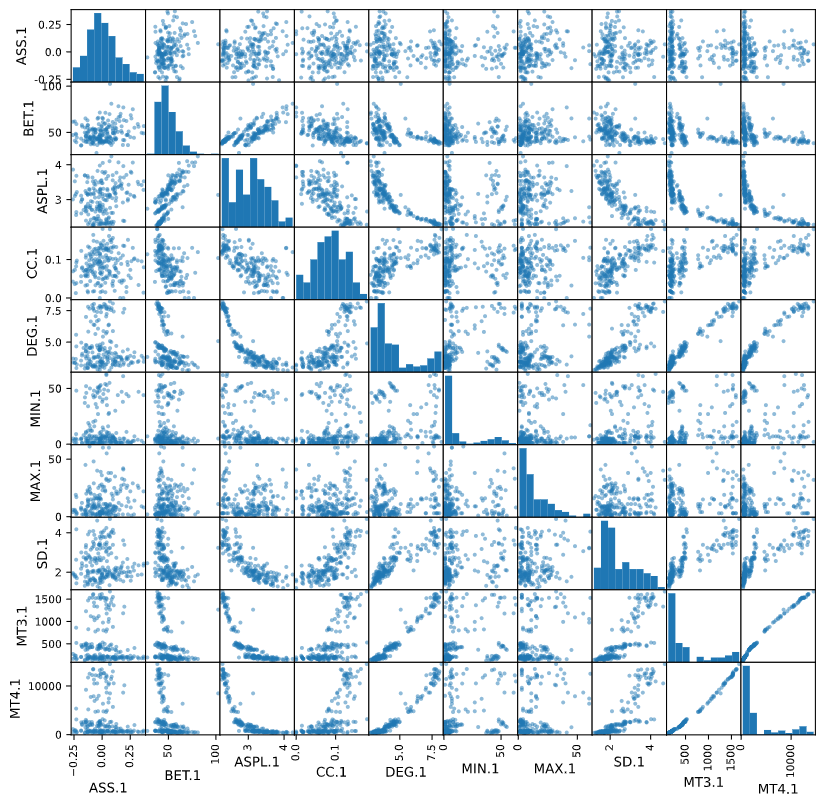
\includegraphics[scale=0.5]{fig/scatter_hist01.png}
 % scatter.png: 619x604 px, 96dpi, 16.38x15.98 cm, bb=0 0 464 453
 \caption{Representação: \textit{Scatter plot} com histograma - Dataset original.}
 \label{fig:scatter_hist01}
\end{figure}

\newpage
\begin{figure}[H]
 \centering
 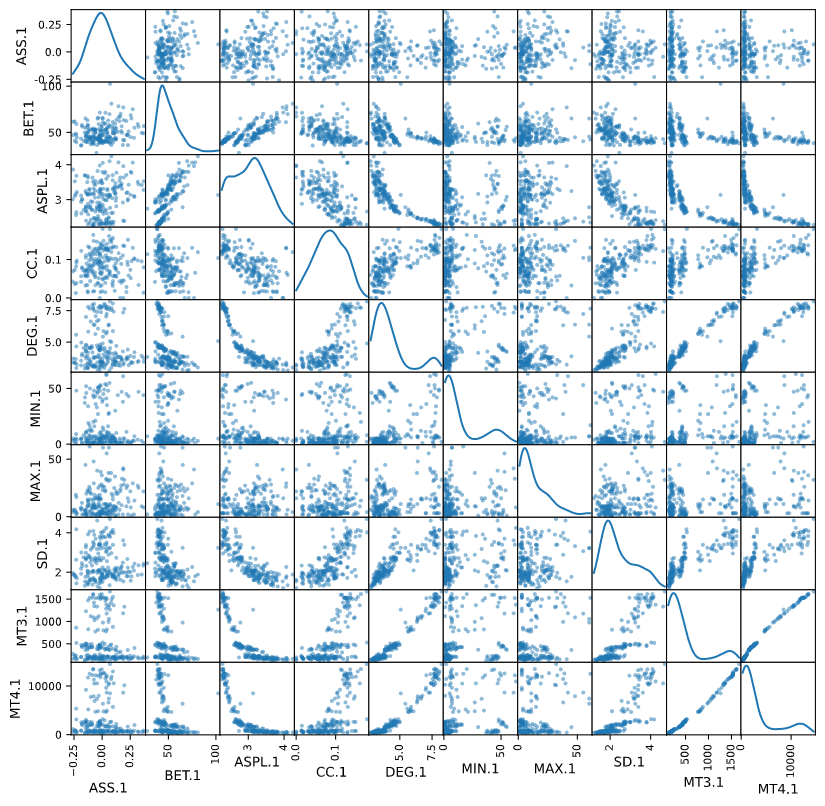
\includegraphics[scale=0.5]{fig/scatter_kde01.png}
 % scatter.png: 619x604 px, 96dpi, 16.38x15.98 cm, bb=0 0 464 453
 \caption{Representação: \textit{Scatter plot} com histograma - Dataset original.}
 \label{fig:scatter_kde01}
\end{figure}

\newpage
\begin{figure}[H]
 \centering
 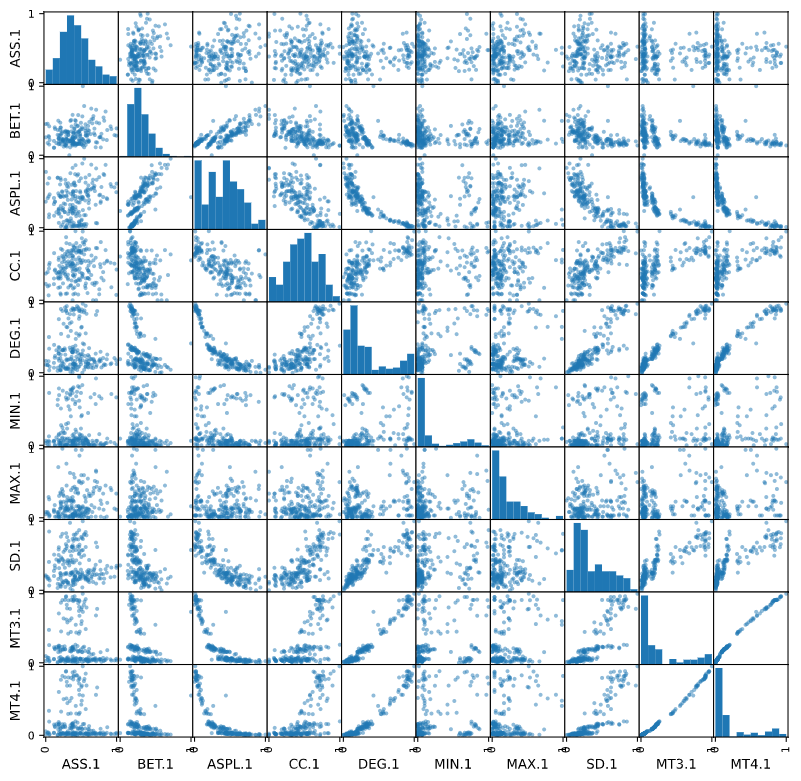
\includegraphics[scale=0.5]{fig/scatter_hist02.png}
 % scatter.png: 619x604 px, 96dpi, 16.38x15.98 cm, bb=0 0 464 453
 \caption{Representação: \textit{Scatter plot} com histograma - Dataset normalizado.}
 \label{fig:scatter_hist02}
\end{figure}

\newpage
\begin{figure}[H]
 \centering
 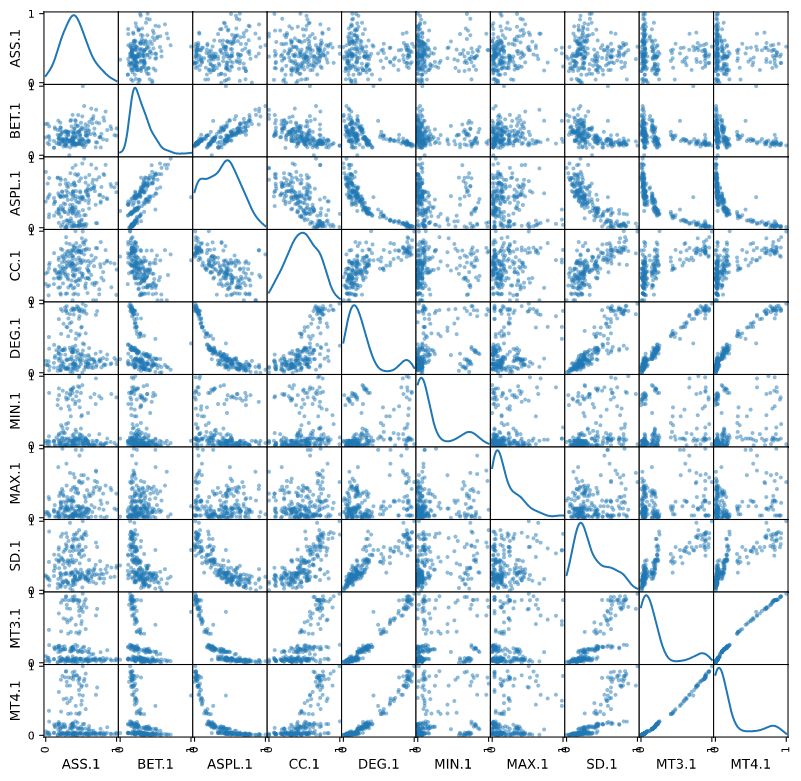
\includegraphics[scale=0.5]{fig/scatter_kde02.png}
 % scatter.png: 619x604 px, 96dpi, 16.38x15.98 cm, bb=0 0 464 453
 \caption{Representação: \textit{Scatter plot} com histograma - Dataset normalizado.}
 \label{fig:scatter_kde02}
\end{figure}

\newpage
\begin{table}[H]
\small
\centering
\begin{tabular}{l|c|c|c|c|c|c|c|c|}
\cline{2-9}
                                      & count   & mean     & std      & min     & 25\%    & 50\%     & 75\%     & max       \\ \hline
\multicolumn{1}{|l|}{\textbf{ASS.1}}  & 200.000 & 0.008    & 0.131    & -0.260  & -0.081  & -0.005   & 0.086    & 0.370     \\ \hline
\multicolumn{1}{|l|}{\textbf{ASS.2}}  & 200.000 & 0.056    & 0.439    & -1.000  & -0.167  & 0.000    & 0.102    & 1.000     \\ \hline
\multicolumn{1}{|l|}{\textbf{ASS.3}}  & 200.000 & -0.008   & 0.153    & -1.000  & 0.000   & 0.000    & 0.000    & 1.000     \\ \hline
\multicolumn{1}{|l|}{\textbf{BET.1}}  & 200.000 & 49.619   & 10.103   & 27.818  & 42.495  & 47.379   & 55.014   & 102.443   \\ \hline
\multicolumn{1}{|l|}{\textbf{BET.2}}  & 200.000 & 0.195    & 0.573    & 0.000   & 0.000   & 0.017    & 0.082    & 4.000     \\ \hline
\multicolumn{1}{|l|}{\textbf{BET.3}}  & 200.000 & 0.001    & 0.008    & 0.000   & 0.000   & 0.000    & 0.000    & 0.078     \\ \hline
\multicolumn{1}{|l|}{\textbf{ASPL.1}} & 200.000 & 3.030    & 0.482    & 2.258   & 2.655   & 3.072    & 3.375    & 4.239     \\ \hline
\multicolumn{1}{|l|}{\textbf{ASPL.2}} & 200.000 & 46.516   & 17.194   & 0.000   & 43.448  & 48.695   & 58.519   & 96.856    \\ \hline
\multicolumn{1}{|l|}{\textbf{ASPL.3}} & 200.000 & 14.922   & 24.588   & 0.000   & 0.000   & 0.000    & 43.204   & 66.940    \\ \hline
\multicolumn{1}{|l|}{\textbf{ASPL.4}} & 200.000 & 1.124    & 7.939    & 0.000   & 0.000   & 0.000    & 0.000    & 62.968    \\ \hline
\multicolumn{1}{|l|}{\textbf{CC.1}}   & 200.000 & 0.085    & 0.039    & 0.000   & 0.058   & 0.086    & 0.115    & 0.180     \\ \hline
\multicolumn{1}{|l|}{\textbf{CC.2}}   & 200.000 & 0.002    & 0.016    & 0.000   & 0.000   & 0.000    & 0.000    & 0.176     \\ \hline
\multicolumn{1}{|l|}{\textbf{DEG.1}}  & 200.000 & 4.560    & 1.603    & 2.739   & 3.383   & 3.861    & 5.018    & 8.230     \\ \hline
\multicolumn{1}{|l|}{\textbf{DEG.2}}  & 200.000 & 0.486    & 0.373    & 0.000   & 0.218   & 0.400    & 0.693    & 1.651     \\ \hline
\multicolumn{1}{|l|}{\textbf{DEG.3}}  & 200.000 & 0.047    & 0.090    & 0.000   & 0.000   & 0.000    & 0.097    & 0.408     \\ \hline
\multicolumn{1}{|l|}{\textbf{DEG.4}}  & 200.000 & 0.004    & 0.026    & 0.000   & 0.000   & 0.000    & 0.000    & 0.258     \\ \hline
\multicolumn{1}{|l|}{\textbf{MIN.1}}  & 200.000 & 14.090   & 17.678   & 1.000   & 3.000   & 5.000    & 16.250   & 63.000    \\ \hline
\multicolumn{1}{|l|}{\textbf{MIN.2}}  & 200.000 & 1.370    & 1.261    & 0.000   & 1.000   & 1.000    & 1.000    & 12.000    \\ \hline
\multicolumn{1}{|l|}{\textbf{MIN.3}}  & 200.000 & 0.280    & 0.461    & 0.000   & 0.000   & 0.000    & 1.000    & 2.000     \\ \hline
\multicolumn{1}{|l|}{\textbf{MIN.4}}  & 200.000 & 0.020    & 0.140    & 0.000   & 0.000   & 0.000    & 0.000    & 1.000     \\ \hline
\multicolumn{1}{|l|}{\textbf{MAX.1}}  & 200.000 & 13.280   & 12.463   & 1.000   & 4.000   & 9.000    & 20.000   & 61.000    \\ \hline
\multicolumn{1}{|l|}{\textbf{MAX.2}}  & 200.000 & 14.210   & 14.217   & 0.000   & 2.000   & 10.500   & 22.000   & 64.000    \\ \hline
\multicolumn{1}{|l|}{\textbf{MAX.3}}  & 200.000 & 4.675    & 9.666    & 0.000   & 0.000   & 0.000    & 5.000    & 61.000    \\ \hline
\multicolumn{1}{|l|}{\textbf{MAX.4}}  & 200.000 & 0.315    & 2.685    & 0.000   & 0.000   & 0.000    & 0.000    & 27.000    \\ \hline
\multicolumn{1}{|l|}{\textbf{SD.1}}   & 200.000 & 2.438    & 0.815    & 1.195   & 1.797   & 2.118    & 3.012    & 4.699     \\ \hline
\multicolumn{1}{|l|}{\textbf{SD.2}}   & 200.000 & 0.969    & 0.526    & 0.000   & 0.668   & 0.977    & 1.312    & 2.627     \\ \hline
\multicolumn{1}{|l|}{\textbf{SD.3}}   & 200.000 & 0.197    & 0.341    & 0.000   & 0.000   & 0.000    & 0.535    & 1.435     \\ \hline
\multicolumn{1}{|l|}{\textbf{SD.4}}   & 200.000 & 0.016    & 0.116    & 0.000   & 0.000   & 0.000    & 0.000    & 0.991     \\ \hline
\multicolumn{1}{|l|}{\textbf{MT3.1}}  & 200.000 & 523.565  & 472.070  & 125.000 & 192.000 & 291.500  & 590.500  & 1669.000  \\ \hline
\multicolumn{1}{|l|}{\textbf{MT3.2}}  & 200.000 & 2.950    & 5.229    & 0.000   & 0.000   & 1.000    & 3.250    & 29.000    \\ \hline
\multicolumn{1}{|l|}{\textbf{MT3.3}}  & 200.000 & 0.050    & 0.313    & 0.000   & 0.000   & 0.000    & 0.000    & 3.000     \\ \hline
\multicolumn{1}{|l|}{\textbf{MT4.1}}  & 200.000 & 3318.465 & 4081.450 & 313.000 & 643.250 & 1180.500 & 3542.000 & 14500.000 \\ \hline
\multicolumn{1}{|l|}{\textbf{MT4.2}}  & 200.000 & 2.490    & 7.193    & 0.000   & 0.000   & 0.000    & 1.000    & 53.000    \\ \hline
\multicolumn{1}{|l|}{\textbf{MT4.3}}  & 200.000 & 0.015    & 0.122    & 0.000   & 0.000   & 0.000    & 0.000    & 1.000     \\ \hline
\end{tabular}
\caption{Medidas de posição e dispersão - Dataset original.}
\label{tab:est_ori}
\end{table}

\newpage
\begin{table}[H]
\centering
\begin{tabular}{l|c|c|c|c|c|c|c|c|}
\cline{2-9}
                                      & count   & mean  & std   & min   & 25\%  & 50\%  & 75\%  & max   \\ \hline
\multicolumn{1}{|l|}{\textbf{ASS.1}}  & 200.000 & 0.425 & 0.207 & 0.000 & 0.284 & 0.404 & 0.549 & 1.000 \\ \hline
\multicolumn{1}{|l|}{\textbf{ASS.2}}  & 200.000 & 0.528 & 0.219 & 0.000 & 0.417 & 0.500 & 0.551 & 1.000 \\ \hline
\multicolumn{1}{|l|}{\textbf{ASS.3}}  & 200.000 & 0.496 & 0.077 & 0.000 & 0.500 & 0.500 & 0.500 & 1.000 \\ \hline
\multicolumn{1}{|l|}{\textbf{BET.1}}  & 200.000 & 0.292 & 0.135 & 0.000 & 0.197 & 0.262 & 0.364 & 1.000 \\ \hline
\multicolumn{1}{|l|}{\textbf{BET.2}}  & 200.000 & 0.049 & 0.143 & 0.000 & 0.000 & 0.004 & 0.021 & 1.000 \\ \hline
\multicolumn{1}{|l|}{\textbf{BET.3}}  & 200.000 & 0.016 & 0.105 & 0.000 & 0.000 & 0.000 & 0.000 & 1.000 \\ \hline
\multicolumn{1}{|l|}{\textbf{ASPL.1}} & 200.000 & 0.390 & 0.243 & 0.000 & 0.200 & 0.411 & 0.564 & 1.000 \\ \hline
\multicolumn{1}{|l|}{\textbf{ASPL.2}} & 200.000 & 0.480 & 0.178 & 0.000 & 0.449 & 0.503 & 0.604 & 1.000 \\ \hline
\multicolumn{1}{|l|}{\textbf{ASPL.3}} & 200.000 & 0.223 & 0.367 & 0.000 & 0.000 & 0.000 & 0.645 & 1.000 \\ \hline
\multicolumn{1}{|l|}{\textbf{ASPL.4}} & 200.000 & 0.018 & 0.126 & 0.000 & 0.000 & 0.000 & 0.000 & 1.000 \\ \hline
\multicolumn{1}{|l|}{\textbf{CC.1}}   & 200.000 & 0.475 & 0.216 & 0.000 & 0.321 & 0.479 & 0.637 & 1.000 \\ \hline
\multicolumn{1}{|l|}{\textbf{CC.2}}   & 200.000 & 0.011 & 0.093 & 0.000 & 0.000 & 0.000 & 0.000 & 1.000 \\ \hline
\multicolumn{1}{|l|}{\textbf{DEG.1}}  & 200.000 & 0.332 & 0.292 & 0.000 & 0.117 & 0.204 & 0.415 & 1.000 \\ \hline
\multicolumn{1}{|l|}{\textbf{DEG.2}}  & 200.000 & 0.294 & 0.226 & 0.000 & 0.132 & 0.242 & 0.420 & 1.000 \\ \hline
\multicolumn{1}{|l|}{\textbf{DEG.3}}  & 200.000 & 0.116 & 0.221 & 0.000 & 0.000 & 0.000 & 0.238 & 1.000 \\ \hline
\multicolumn{1}{|l|}{\textbf{DEG.4}}  & 200.000 & 0.014 & 0.100 & 0.000 & 0.000 & 0.000 & 0.000 & 1.000 \\ \hline
\multicolumn{1}{|l|}{\textbf{MIN.1}}  & 200.000 & 0.211 & 0.285 & 0.000 & 0.032 & 0.065 & 0.246 & 1.000 \\ \hline
\multicolumn{1}{|l|}{\textbf{MIN.2}}  & 200.000 & 0.114 & 0.105 & 0.000 & 0.083 & 0.083 & 0.083 & 1.000 \\ \hline
\multicolumn{1}{|l|}{\textbf{MIN.3}}  & 200.000 & 0.140 & 0.231 & 0.000 & 0.000 & 0.000 & 0.500 & 1.000 \\ \hline
\multicolumn{1}{|l|}{\textbf{MIN.4}}  & 200.000 & 0.020 & 0.140 & 0.000 & 0.000 & 0.000 & 0.000 & 1.000 \\ \hline
\multicolumn{1}{|l|}{\textbf{MAX.1}}  & 200.000 & 0.205 & 0.208 & 0.000 & 0.050 & 0.133 & 0.317 & 1.000 \\ \hline
\multicolumn{1}{|l|}{\textbf{MAX.2}}  & 200.000 & 0.222 & 0.222 & 0.000 & 0.031 & 0.164 & 0.344 & 1.000 \\ \hline
\multicolumn{1}{|l|}{\textbf{MAX.3}}  & 200.000 & 0.077 & 0.158 & 0.000 & 0.000 & 0.000 & 0.082 & 1.000 \\ \hline
\multicolumn{1}{|l|}{\textbf{MAX.4}}  & 200.000 & 0.012 & 0.099 & 0.000 & 0.000 & 0.000 & 0.000 & 1.000 \\ \hline
\multicolumn{1}{|l|}{\textbf{SD.1}}   & 200.000 & 0.355 & 0.233 & 0.000 & 0.172 & 0.263 & 0.518 & 1.000 \\ \hline
\multicolumn{1}{|l|}{\textbf{SD.2}}   & 200.000 & 0.369 & 0.200 & 0.000 & 0.254 & 0.372 & 0.499 & 1.000 \\ \hline
\multicolumn{1}{|l|}{\textbf{SD.3}}   & 200.000 & 0.137 & 0.238 & 0.000 & 0.000 & 0.000 & 0.373 & 1.000 \\ \hline
\multicolumn{1}{|l|}{\textbf{SD.4}}   & 200.000 & 0.017 & 0.117 & 0.000 & 0.000 & 0.000 & 0.000 & 1.000 \\ \hline
\multicolumn{1}{|l|}{\textbf{MT3.1}}  & 200.000 & 0.258 & 0.306 & 0.000 & 0.043 & 0.108 & 0.301 & 1.000 \\ \hline
\multicolumn{1}{|l|}{\textbf{MT3.2}}  & 200.000 & 0.102 & 0.180 & 0.000 & 0.000 & 0.034 & 0.112 & 1.000 \\ \hline
\multicolumn{1}{|l|}{\textbf{MT3.3}}  & 200.000 & 0.017 & 0.104 & 0.000 & 0.000 & 0.000 & 0.000 & 1.000 \\ \hline
\multicolumn{1}{|l|}{\textbf{MT4.1}}  & 200.000 & 0.212 & 0.288 & 0.000 & 0.023 & 0.061 & 0.228 & 1.000 \\ \hline
\multicolumn{1}{|l|}{\textbf{MT4.2}}  & 200.000 & 0.047 & 0.136 & 0.000 & 0.000 & 0.000 & 0.019 & 1.000 \\ \hline
\multicolumn{1}{|l|}{\textbf{MT4.3}}  & 200.000 & 0.015 & 0.122 & 0.000 & 0.000 & 0.000 & 0.000 & 1.000 \\ \hline
\end{tabular}
\caption{Medidas de posição e dispersão - Dataset normalizado.}
\label{tab:est_norm}
\end{table}

\newpage
\begin{figure}[H]
 \centering
 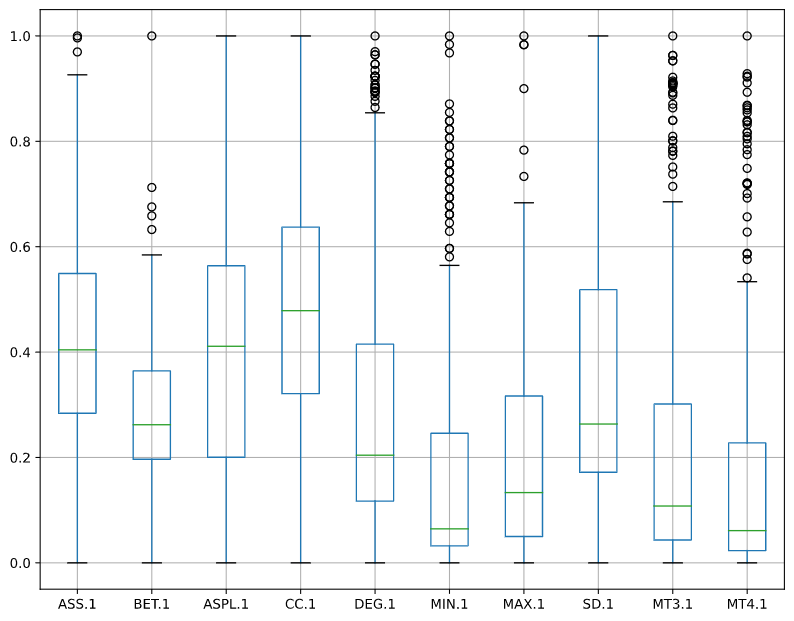
\includegraphics[scale=0.4]{fig/boxplot.png}
 % scatter.png: 619x604 px, 96dpi, 16.38x15.98 cm, bb=0 0 464 453
 \caption{\textit{Boxplot} de $10$ características - Dataset normalizado.}
 \label{fig:boxplot}
\end{figure}

\begin{figure}[H]
 \centering
 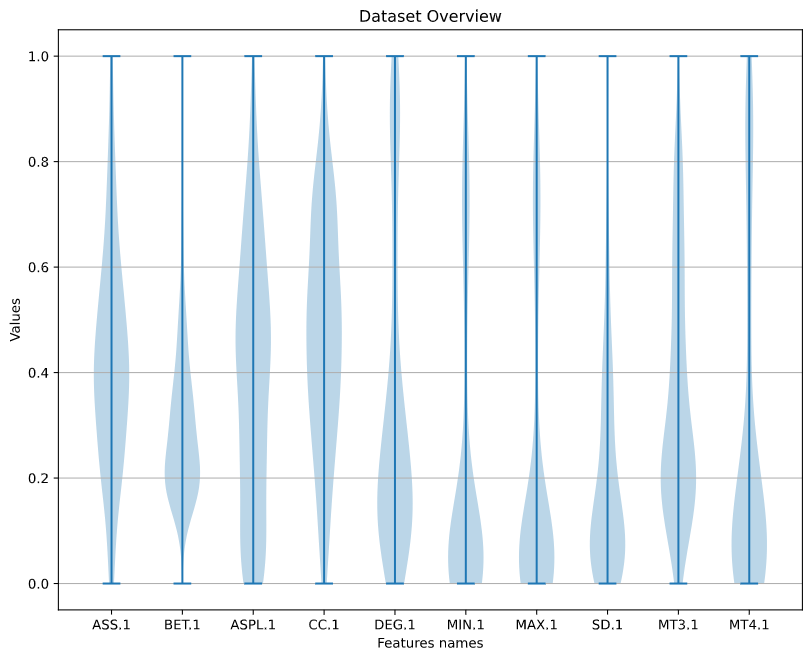
\includegraphics[scale=0.4]{fig/violin.png}
 % scatter.png: 619x604 px, 96dpi, 16.38x15.98 cm, bb=0 0 464 453
 \caption{\textit{Violin plot} de $10$ características - Dataset normalizado.}
 \label{fig:violin}
\end{figure}

\newpage
\section{Classificadores}

O objetivo deste trabalho é apresentar a execução de alguns classificadores, dessa forma optou-se por utilizar $6$ classificadores e um dataset pequeno, devido as limitações de hardware para as execuções, logo não foram considerados classificadores do tipo \textit{ deep learning}. A escolha do dataset não afeta o objetivo ante exposto. Algumas observações em relação aos resultados obtidos são necessárias já que o dataset é pequeno para análises detalhadas sobre os resultados obtidos. Dessa maneira os resultados apresentados estão restritos a este dataset, para uma generalização é necessário um conjunto de dados maior.

O dataset foi binarizado e separado de maneira estratificada em conjuntos de treinamento e teste na seguinte proporção, $80\%$ dos dados para treinamento e $20\%$ para teste. A biblioteca \verb|sklearn| foi utilizada nesta etapa.

\begin{verbatim}
 #Binarizando os dados
 Y_bin = label_binarize(df['CLASS'], 
                       classes=class_label)
 
 #Split dataset
 X_train, X_test, y_train, y_test = train_test_split(X,
                                                    Y_bin, 
                                                    test_size=0.2,
                                                    stratify=class_names)
 y_true = np.argmax(y_test, axis = 1)
\end{verbatim}


\subsection{k-nearest neighbors $(k-NN)$}

O classificador k-nearest neighbors foi proposto inicialmente na década de $60$, e expandido na década de $90$ \cite{KNN}. A proposta do algoritmo é realizar a comparação da distância da $i$-ésima amostra com $k$ vizinhos mais próximos e através de votação classificar a amostra como pertencente a classe de maior votos. Os parâmetros utilizados pelo algoritmo são os seguintes:
\begin{itemize}
 \item A métrica para o cálculo da distância,
 \item O valor de $k$, isto é, quantos vizinhos serão considerados para a comparação.
\end{itemize}

As métricas mais utilizadas são a distância Euclidiana (eq. \ref{eq: dist1}), de Minkowsky (eq. \ref{eq: dist2}) e Chebyshev (eq. \ref{eq: dist3}).

\begin{align}
 \label{eq: dist1}
  d_E\left( p,q\right)&= \sqrt {\sum _{i=1}^{n}  \left( q_{i}-p_{i}\right)^2 } \\
  \label{eq: dist2}
  D_M\left( p,q\right)&= \left( \sum_{i=1}^{n} \left| p_i - q_i \right|^r \right)^{\frac{1}{r}} 
  \\
  \label{eq: dist3}
  D_C\left( p,q\right)&= \max_i(|p_i,q_i|) 
\end{align}

Já o valor de $k$ é um valor a ser definido através de heurísticas para a seleção de melhores valores, neste projeto optou-se por realizar um refinamento do algoritmo utilizando a abordagem \textit{grid}.

\begin{figure}[H]
 \centering
 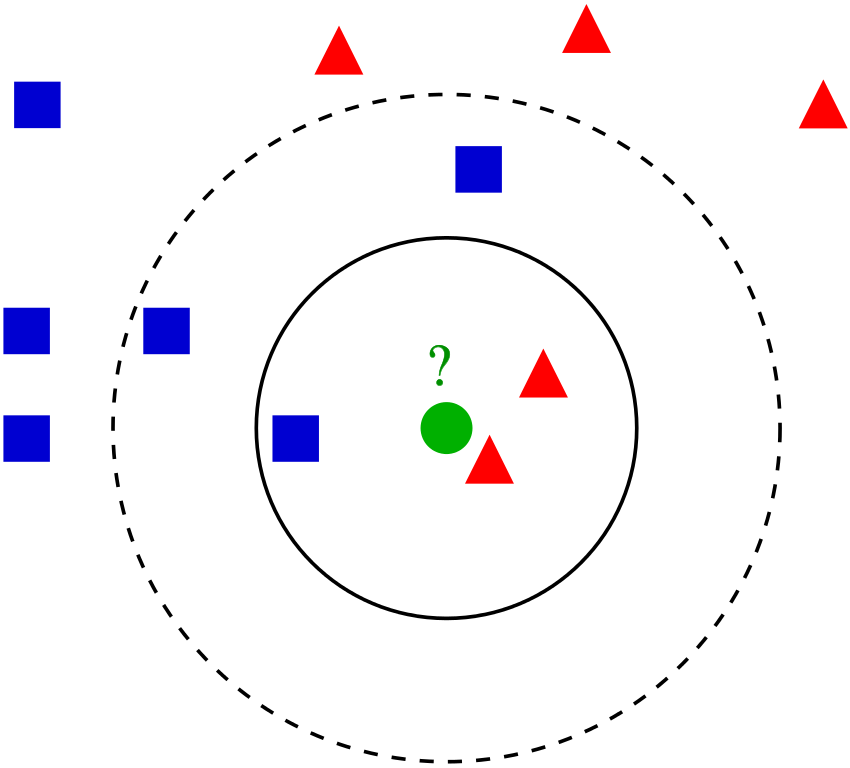
\includegraphics[scale=0.2]{fig/knn_alg.png}
 % scatter.png: 619x604 px, 96dpi, 16.38x15.98 cm, bb=0 0 464 453
 \caption{Exemplo de classificação utilizando $k-NN$, o círculo verde é um novo elemento para classificação, caso seja considerado $k=3$ (círculo preto contínuo) a classe do elemento verde é a mesma dos elementos vermelhos, por outro lado considerando $k=5$ temos que a classe escolhido é a mesma dos elementos azuis, já que são maioria dentre este intervalo. Fonte: Antti Ajanki sob CC BY-SA 3.0}
 \label{fig:knn_alg}
\end{figure}

O algoritmo utilizado esta implementado no pacote \verb|sklearn.neighbors|, com a métrica padrão Euclidiana. Inicialmente com o valor de $k=3$ foi utilizado para a análise dos resultados.

\begin{verbatim}
 #file: knn.ipynb
 knn = KNeighborsClassifier(n_neighbors=3)
 knn.fit(X_train, y_train)
 knn3_res = knn.predict(X_test)
 y_pred_knn3 = np.argmax(knn3_res, axis=1)
\end{verbatim}

As métricas obtidas para o valor de $k=3$ são apresentadas na tabela \ref{tab:knn_01}.

\begin{verbatim}
 #file: knn.ipynb
 #Matriz de confusão
 KNN3_cm = confusion_matrix(y_true=y_true, 
                           y_pred=y_pred_knn3)
 #heatmap                           
 plt.figure(figsize = (10,8))
 ax = plt.axes()
 x_axis_labels = ['class_1', 'class_2', 'class_3', 'class_4'] # labels for
 x-axis
 y_axis_labels = ['class_1', 'class_2', 'class_3', 'class_4'] # labels for 
 y-axis
 sns.heatmap(KNN3_cm,
             vmin=0,
             vmax=10,
             annot=True,
             fmt="d",
             ax = ax,
             xticklabels=x_axis_labels, 
             yticklabels=y_axis_labels)
 ax.set_title('Heatmap for KNN Classification Model',pad=15)
\end{verbatim}

\begin{table}[H]
\centering
\begin{tabular}{l|c|c|c|c|}
\cline{2-5}
                                            & \textbf{precision} & \textbf{recall} & \textbf{f1-score} & \textbf{support} \\ \hline
\multicolumn{1}{|l|}{\textbf{class\_1}}     & 0.71               & 1.00            & 0.83              & 10               \\ \hline
\multicolumn{1}{|l|}{\textbf{class\_2}}     & 1.00               & 1.00            & 1.00              & 10               \\ \hline
\multicolumn{1}{|l|}{\textbf{class\_3}}     & 0.75               & 0.30            & 0.43              & 10               \\ \hline
\multicolumn{1}{|l|}{\textbf{class\_4}}     & 0.75               & 0.90            & 0.82              & 10               \\ \hline
\multicolumn{1}{|l|}{\textbf{accuracy}}     &                    &                 & 0.80              & 40               \\ \hline
\multicolumn{1}{|l|}{\textbf{macro avg}}    & 0.80               & 0.80            & 0.77              & 40               \\ \hline
\multicolumn{1}{|l|}{\textbf{weighted avg}} & 0.80               & 0.80            & 0.77              & 40               \\ \hline
\end{tabular}
\caption{Métricas - $k-NN$ - $k=3$}
\label{tab:knn_01}
\end{table}

E a seguinte matriz de confusão (Figura \ref{fig:knn_cm01}):

\begin{figure}[H]
 \centering
 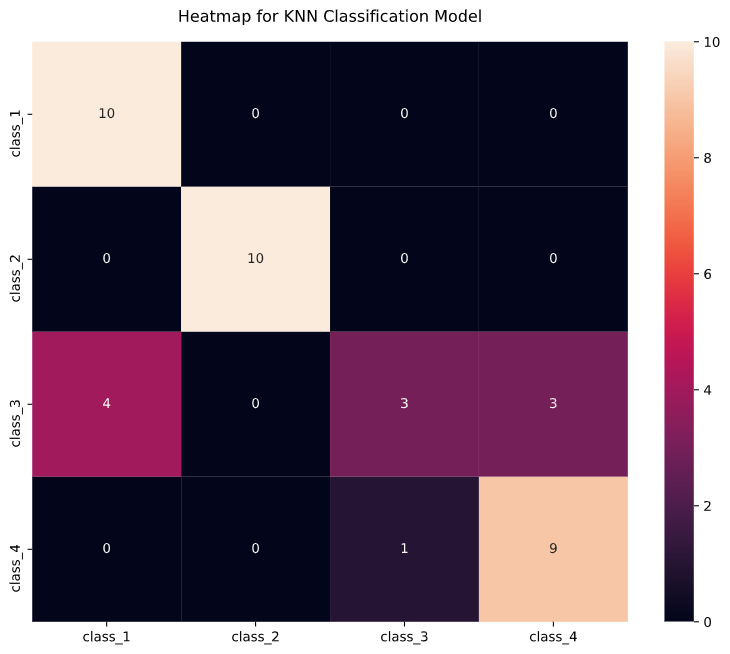
\includegraphics[scale=0.35]{fig/knn_cm01.png}
 % scatter.png: 619x604 px, 96dpi, 16.38x15.98 cm, bb=0 0 464 453
 \caption{Matriz de confusão e heatmap para o conjunto de teste utilizando o classificador $k-NN$ - $k=3$.}
 \label{fig:knn_cm01}
\end{figure}

Com o objetivo de obter um melhor valor da acurácia, foi realizada uma busca em $grid$ para selecionar o melhor valor de $k$ em um intervalo de $[1,30]$ utilizando uma validação cruzada de $10-fold$. Utilizou-se dessa abordagem como forma de mostrar que o classificador possui parâmetros que devem ser ajustados conforme o dataset utilizado. 

\begin{verbatim}
 #file: knn.ipynb
 #Intervalo de busca
 k_list = list(range(1,31))
 knn_param = dict(n_neighbors=k_list)
 #grid
 grid = GridSearchCV(knn,
                    knn_param, 
                    cv=10, 
                    scoring='accuracy')
 #Fit
 grid.fit(X_train, y_train)
 #Print
 print("Melhores parametros {} com o valor de acurácia {}
 ".format(grid.best_params_,grid.best_score_))
\end{verbatim}


Os seguintes valores de acurácias médias para cada uma das execuções das validações cruzados são exibidos na figura \ref{fig:knn_grid}. Neste caso, em particular, a maior acurácia utilizando validação cruzada foi obtida com o valor de $k=1$, isto significa que a classe a ser escolhida por um novo elemento será a classe do elemento mais próximo a este novo elemento.

\begin{verbatim}
 #file: knn.ipynb
 knn = KNeighborsClassifier(n_neighbors=1)
 knn.fit(X_train, y_train)
 knn1_res = knn.predict(X_test)
 y_pred_knn1 = np.argmax(knn1_res, axis=1)
 y_predp_knn1 = knn.predict_proba(X_test)
\end{verbatim}


\begin{figure}[H]
 \centering
 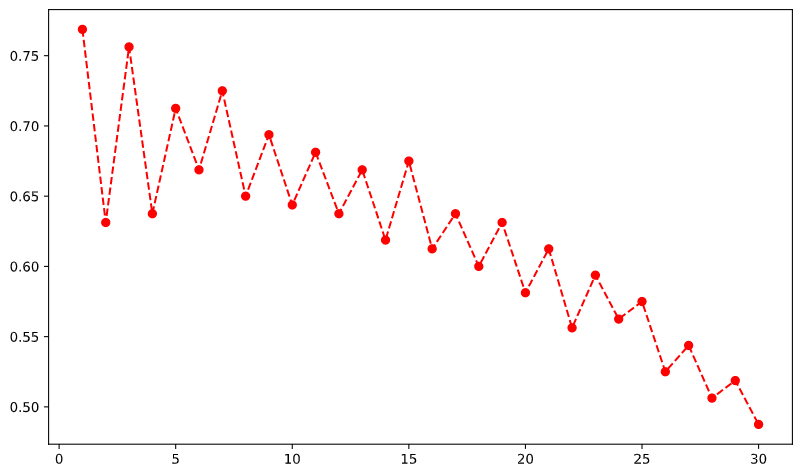
\includegraphics[scale=0.5]{fig/knn_grid.png}
 % scatter.png: 619x604 px, 96dpi, 16.38x15.98 cm, bb=0 0 464 453
 \caption{Acurácias (eixo $y$) obtidas através da variação do valor de $k$ (eixo $x$).}
 \label{fig:knn_grid}
\end{figure}

Utilizando o valor da maior acurácia obtido nas validações cruzadas ($k=1$), as seguintes métricas (Tabela \ref{tab:knn_02}) e matriz de confusão (Figura \ref{fig:knn_cm02}) foram obtidas:

\begin{verbatim}
 #file: knn.ipynb
 KNN1_cm = confusion_matrix(y_true=y_true, 
                           y_pred=y_pred_knn1)
 print(classification_report(y_true, y_pred_knn1, target_names=class_label))
 print(accuracy_score(y_true, y_pred_knn1))                           
\end{verbatim}

\begin{table}[H]
\centering
\begin{tabular}{l|c|c|c|c|}
\cline{2-5}
                                            & \multicolumn{1}{l|}{\textbf{precision}} & \textbf{recall} & \textbf{f1-score} & \textbf{support} \\ \hline
\multicolumn{1}{|l|}{\textbf{class\_1}}     & 0.75                                    & 0.90            & 0.82              & 10               \\ \hline
\multicolumn{1}{|l|}{\textbf{class\_2}}     & 0.91                                    & 1.00            & 0.95              & 10               \\ \hline
\multicolumn{1}{|l|}{\textbf{class\_3}}     & 0.80                                    & 0.40            & 0.53              & 10               \\ \hline
\multicolumn{1}{|l|}{\textbf{class\_4}}     & 0.75                                    & 0.90            & 0.82              & 10               \\ \hline
\multicolumn{1}{|l|}{\textbf{accuracy}}     &                                         &                 & 0.80              & 40               \\ \hline
\multicolumn{1}{|l|}{\textbf{macro avg}}    & 0.80                                    & 0.80            & 0.78              & 40               \\ \hline
\multicolumn{1}{|l|}{\textbf{weighted avg}} & 0.80                                    & 0.80            & 0.78              & 40               \\ \hline
\end{tabular}
\caption{Métricas - $k-NN$ - $k=1$}
\label{tab:knn_02}
\end{table}

\begin{figure}[H]
 \centering
 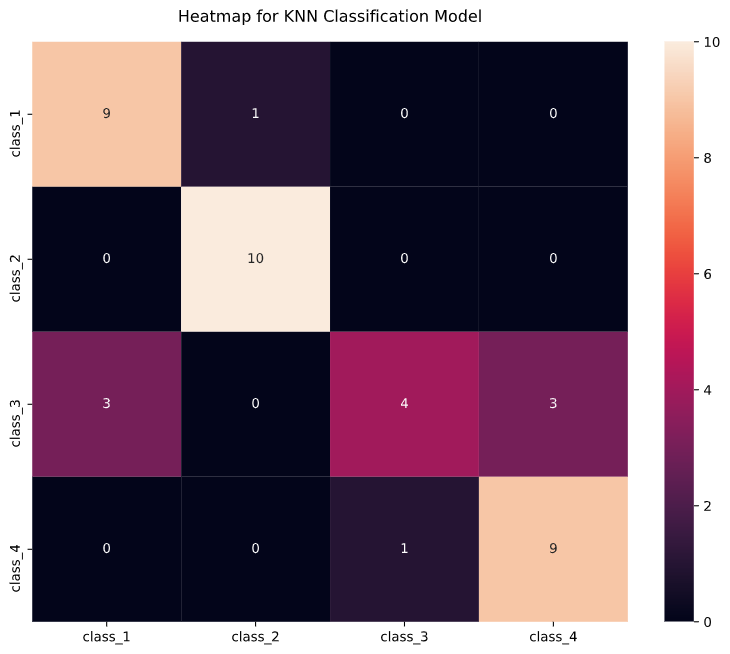
\includegraphics[scale=0.35]{fig/knn_cm02.png}
 % scatter.png: 619x604 px, 96dpi, 16.38x15.98 cm, bb=0 0 464 453
 \caption{Matriz de confusão e heatmap para o conjunto de teste - $k-NN$ - $k=1$.}
 \label{fig:knn_cm02}
\end{figure}

A análise da performance de classificadores pode ser feita analisando a área abaixo da curva ROC (Receiver Operating Characteristic). Quanto maior for a área, isto é, mais próxima a $1$, melhor é a performance do classificador. Como o dataset é multi classe foi utilizada a abordagem ``um contra todos'' para a obtenção das curvas ROC para cada uma das classes, como mostra a figura \ref{knn_roc}.

\begin{verbatim}
 #file: knn.ipynb
 #OneVsRestClassifier
 clf = OneVsRestClassifier(KNeighborsClassifier(n_neighbors=1))
 y_pred_ovr_knn1 = clf.fit(X_train, y_train).predict_proba(X_test)
 #Curva ROC para cada classe
 fpr_KNN1 = dict()
 tpr_KNN1 = dict()
 roc_auc_KNN1 = dict()
 for i in range(class_label.shape[0]):
    fpr_KNN1[i], tpr_KNN1[i], _ = roc_curve(y_test[:, i], y_pred_ovr_knn1[:,
    i])
    roc_auc_KNN1[i] = auc(fpr_KNN1[i], tpr_KNN1[i])
 #Plot
 for i in range(class_label.shape[0]):
    plt.figure()
    plt.plot(fpr_KNN1[i], tpr_KNN1[i], label='ROC curve (area = %0.2f)' %
    roc_auc_KNN1[i])
    plt.plot([0, 1], [0, 1], 'k--')
    plt.xlim([0.0, 1.0])
    plt.ylim([0.0, 1.05])
    plt.xlabel('False Positive Rate')
    plt.ylabel('True Positive Rate')
    plt.title('Receiver operating characteristic (ROC) for %s' %
    class_label[i])
    plt.legend(loc="lower right")
    plt.show()
\end{verbatim}


\begin{figure}[H]
    \centering
    \begin{subfigure}[b]{0.475\textwidth}
    \centering
    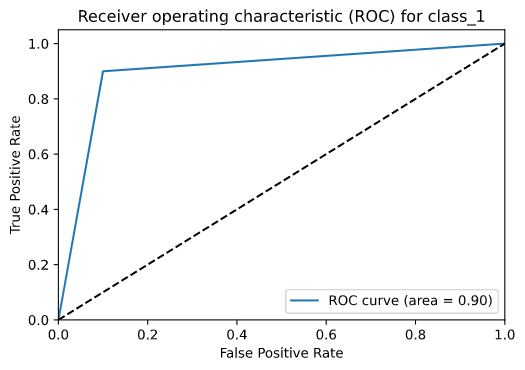
\includegraphics[scale=0.375]{fig/knn_roc1.png}
    \caption{Receiver operating characteristic (ROC) - $class_1$}
    \label{fig:knn_roc1}
    \end{subfigure}
    \hfill
    \begin{subfigure}[b]{0.475\textwidth}
    \centering
    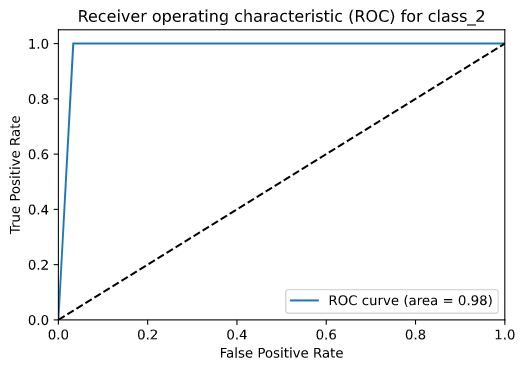
\includegraphics[scale=0.375]{fig/knn_roc2.png}
    \caption{Receiver operating characteristic (ROC) - $class_2$}
    \label{fig:knn_roc2}
    \end{subfigure}
    \vskip\baselineskip
    \begin{subfigure}[b]{0.475\textwidth}
    \centering
    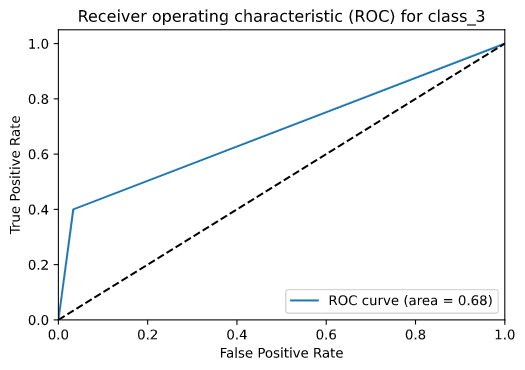
\includegraphics[scale=0.375]{fig/knn_roc3.png}
    \caption{Receiver operating characteristic (ROC) - $class_3$}
    \label{fig:knn_roc3}
    \end{subfigure}
    \hfill
    \begin{subfigure}[b]{0.475\textwidth}
    \centering
    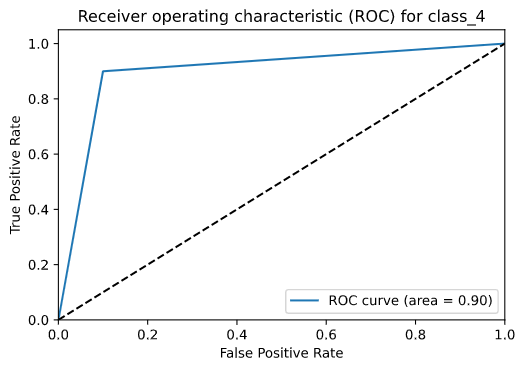
\includegraphics[scale=0.375]{fig/knn_roc4.png}
    \caption{Receiver operating characteristic (ROC) - $class_4$}
    \label{fig:knn_roc4}
    \end{subfigure}
    \caption{Receiver operating characteristic (ROC) para o classificador $k-NN$ com $k=1$.}
    \label{knn_roc}
\end{figure}

O valor do coeficiente Kappa \cite{kappa} é uma métrica que busca avaliar concordância entre conjuntos, no caso de classificadores são analisados os conjuntos de teste e preditos, quanto mais próximo de $1$, maior é o nível de concordância entre os conjuntos. Para $k-NN$ com $k=1$ o valor do coeficiente de Kappa é $0.73$ com as seguintes métricas (Tabela \ref{tab:metrics_knn}).

\begin{verbatim}
 #file: knn.ipynb
 #Kappa
 knn_kappa = cohen_kappa_score(y_true, y_pred_knn1)
\end{verbatim}

\begin{table}[H]
\centering
\begin{tabular}{|l|c|c|c|c|}
\hline
\multicolumn{1}{|c|}{\textbf{Métrica}} & \textbf{Class1} & \textbf{Class2} & \textbf{Class3} & \textbf{Class4} \\ \hline
\textbf{Sensibilidade:}                & 0.9             & 1               & 0.4             & 0.9             \\ \hline
\textbf{True Negative:}                & 0.9             & 0.96            & 0.96            & 0.9             \\ \hline
\textbf{Precisão:}                     & 0.75            & 0.9             & 0.8             & 0.75            \\ \hline
\textbf{Pred. Negativa:}               & 0.96            & 1               & 0.82            & 0.96            \\ \hline
\textbf{False Positive:}               & 0.1             & 0.03            & {]}0.03         & 0.1             \\ \hline
\textbf{False Negative:}               & 0.1             & 0               & 0.6             & 0.1             \\ \hline
\textbf{False Discovery:}              & 0.25            & 0.09            & 0.2             & 0.25            \\ \hline
\textbf{Acurácia:}                     & 0.9             & 0.97            & 0.82            & 0.9             \\ \hline
\end{tabular}
\caption{Métricas - $k-NN$ - $k=1$}
\label{tab:metrics_knn}
\end{table}

\subsection{Árvore de Decisão}

O classificador árvore de decisão busca relacionar os atributos (características) dos elementos (observações) com seus respectivos rótulos (classes) utilizando uma estrutura de grafos em topologia de árvore \cite{Safavian1991}. O objetivo é identificar quais as melhores características para realizar a ``divisão'' dos dados nas classes corretas.

Para isso são considerados algumas métricas que buscam mensurar quão nítida pode ser essa divisão, como por exemplo a métrica de Gini ou ainda o quanto de informação é recebido com as divisões, através do cálculo de entropia.

É um método ``simples'', não exigindo conhecimentos prévios a respeito dos dados, contudo altamente propenso a \textit{overfitting} dos dados de treinamento. Alternativas a este comportamento são propostas nos classificadores seguintes.

\begin{figure}
\begin{center}
\begin{tikzpicture}[
    fact/.style={rectangle, draw=none, rounded corners=1mm, fill=blue, drop shadow,
        text centered, anchor=north, text=white},
    state/.style={circle, draw=none, fill=orange, circular drop shadow,
        text centered, anchor=north, text=white},
    leaf/.style={circle, draw=none, fill=red, circular drop shadow,
        text centered, anchor=north, text=white},
    level distance=0.5cm, growth parent anchor=south
]
\node (State00) [state] {$S_{00}$} [->]
    child{
        node (Fact01) [fact] {$T_{01}$}
        child{ [sibling distance=9cm]
            node (State01) [state] {$S_{01}$}
            child{
                node (Fact02) [fact] {$T_{02}$}
                child{ [sibling distance=4cm]
                    node (State02) [state] {$S_{02}$}
                    child{
                        node (Fact03) [fact] {$T_{03}$}
                        child{
                            node (State03) [leaf] {$S_{03}$}
                        }
                    }
                    child{
                        node (Fact04) [fact] {$T_{04}$}
                        child{ [sibling distance=1.2cm]
                            node (State04) [state] {$S_{04}$}
                            child{
                                node (Fact05) [fact] {$T_{05}$}
                                child{
                                    node (State05) [leaf] {$S_{05}$}
                                }
                            }
                            child{
                                node (Fact06) [fact] {$T_{06}$}
                                child{
                                    node (State06) [leaf] {$S_{06}$}
                                }
                            }
                            child{
                                node (Fact07) [fact] {$T_{07}$}
                                child{
                                    node (State07) [leaf] {$S_{07}$}
                                }
                            }
                            child{
                                node (Fact08) [fact] {$T_{08}$}
                                child{
                                    node (State08) [leaf] {$S_{08}$}
                                }
                            }
                            child{
                                node (Fact09) [fact] {$T_{09.0}$}
                                child{
                                    node (Fact09-1) [fact] {$T_{09.1}$}
                                    child{
                                        node (State09) [leaf] {$S_{09}$}
                                    }
                                }
                            }
                        }
                    }
                }
            }
            child{ [sibling distance=4cm]
                node (Fact10) [fact] {$T_{10}$}
                child{
                    node (State10) [state] {$S_{10}$}
                    child{
                        node (Fact11) [fact] {$T_{11}$}
                        child{
                            node (State11) [leaf] {$S_{11}$}
                        }
                    }
                }
            }
        }
    }   
;
 
\end{tikzpicture}
\end{center}
\label{ex_dt}
 \caption{Exemplo de árvore de decisão, com o nó raiz acima $(S_{00})$ e a partir dele os ramos (características) e folhas em vermelho (rótulos) das classificações.}
\end{figure}


O algoritmo utilizado está implementado no pacote \verb|tree| da biblioteca \verb|sklearn| com o seguinte método \verb|DecisionTreeClassifier|. Os parâmetros utilizados foram configurados com os valores \textit{default} do pacote.

\begin{verbatim}
 #file: dt.ipynb
 DT = tree.DecisionTreeClassifier()
 DT.fit(X_train,y_train)
 DT_res = DT.predict(X_test)
 y_pred_DT = np.argmax(DT_res, axis=1)
 y_predp_DT = DT.predict_proba(X_test)
\end{verbatim}

As métricas (Tabela \ref{tab:dt_01}), matriz de confusão (Figura \ref{fig:dt_cm}) e curvas ROC (Figura \ref{dt_roc}) para cada uma das classes são apresentadas a seguir.

\begin{verbatim}
 #file: dt.ipynb
 #Matriz de confusão
 DT_cm = confusion_matrix(y_true=y_true, 
                         y_pred=y_pred_DT)
 #Heatmap
 plt.figure(figsize = (10,8))
 ax = plt.axes()
 x_axis_labels = ['class_1', 'class_2', 'class_3', 'class_4'] # labels for
 x-axis
 y_axis_labels = ['class_1', 'class_2', 'class_3', 'class_4'] # labels for
 y-axis
 sns.heatmap(DT_cm,
             vmin=0,
             vmax=10,
             annot=True,
             fmt="d",
             ax = ax,
             xticklabels=x_axis_labels, 
             yticklabels=y_axis_labels)
 ax.set_title('Heatmap for Decision Tree Classification Model',pad=15)
 #Métricas
 print(classification_report(y_true, y_pred_DT, target_names=class_label))
 print("Accuracy:",metrics.accuracy_score(y_true, y_pred_DT))
 #Curva ROC
 fpr_DT = dict()
 tpr_DT = dict()
 roc_auc_DT = dict()
 for i in range(class_label.shape[0]):
     fpr_DT[i], tpr_DT[i], _ = roc_curve(y_test[:, i], y_pred_ovr_DT[:, i])
     roc_auc_DT[i] = auc(fpr_DT[i], tpr_DT[i])
 #Plot
 for i in range(class_label.shape[0]):
    plt.figure()
    plt.plot(fpr_DT[i], tpr_DT[i], label='ROC curve (area = %0.2f)' % roc_auc_DT[i])
    plt.plot([0, 1], [0, 1], 'k--')
    plt.xlim([0.0, 1.0])
    plt.ylim([0.0, 1.05])
    plt.xlabel('False Positive Rate')
    plt.ylabel('True Positive Rate')
    plt.title('Receiver operating characteristic (ROC) for %s' % class_label[i])
    plt.legend(loc="lower right")
    plt.show()
\end{verbatim}

\newpage
\begin{table}[H]
\centering
\begin{tabular}{c|c|c|c|c|}
\cline{2-5}
                                            & \textbf{precision} & \textbf{recall} & \textbf{f1-score} & \textbf{support} \\ \hline
\multicolumn{1}{|c|}{\textbf{class\_1}}     & 1.00               & 1.00            & 1.00              & 10               \\ \hline
\multicolumn{1}{|c|}{\textbf{class\_2}}     & 1.00               & 1.00            & 1.00              & 10               \\ \hline
\multicolumn{1}{|c|}{\textbf{class\_3}}     & 0.73               & 0.80            & 0.76              & 10               \\ \hline
\multicolumn{1}{|c|}{\textbf{class\_4}}     & 0.78               & 0.70            & 0.74              & 10               \\ \hline
\multicolumn{1}{|c|}{\textbf{accuracy}}     &                    &                 & 0.88              & 40               \\ \hline
\multicolumn{1}{|c|}{\textbf{macro avg}}    & 0.88               & 0.88            & 0.87              & 40               \\ \hline
\multicolumn{1}{|c|}{\textbf{weighted avg}} & 0.88               & 0.88            & 0.87              & 40               \\ \hline
\end{tabular}
\caption{Métricas - Árvore de Decisão}
\label{tab:dt_01}
\end{table}


\begin{figure}[H]
 \centering
 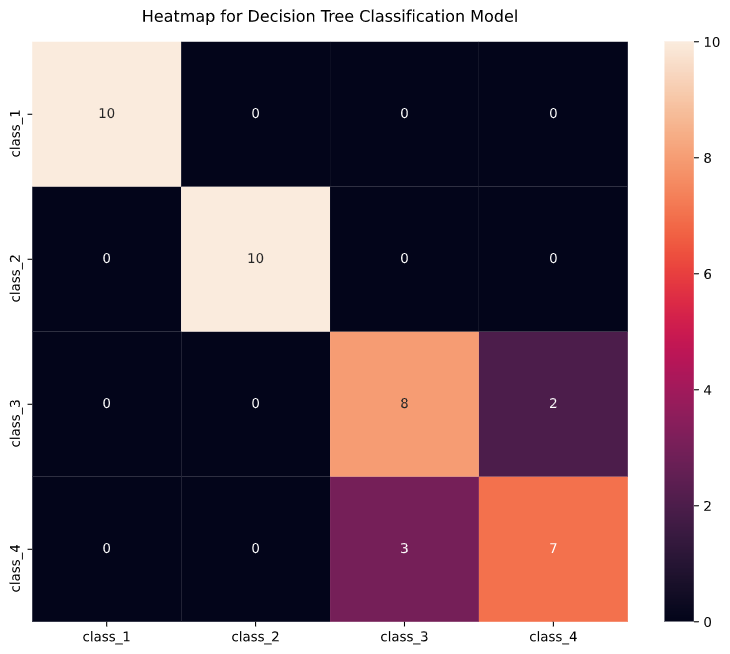
\includegraphics[scale=0.35]{fig/dt_cm.png}
 % scatter.png: 619x604 px, 96dpi, 16.38x15.98 cm, bb=0 0 464 453
 \caption{Matriz de confusão e heatmap para o conjunto de teste - Árvore de Decisão.}
 \label{fig:dt_cm}
\end{figure}

\begin{figure}
    \centering
    \begin{subfigure}[b]{0.475\textwidth}
    \centering
    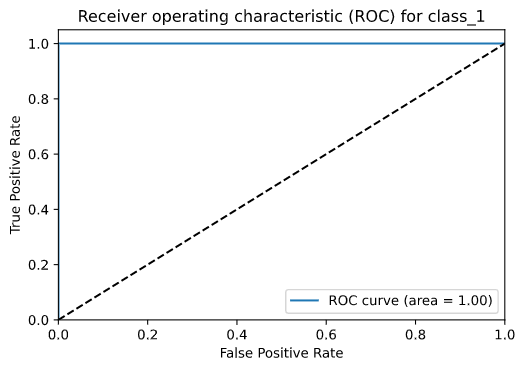
\includegraphics[scale=0.375]{fig/dt_roc1.png}
    \caption{Receiver operating characteristic (ROC) - $class_1$}
    \label{fig:dt_roc1}
    \end{subfigure}
    \hfill
    \begin{subfigure}[b]{0.475\textwidth}
    \centering
    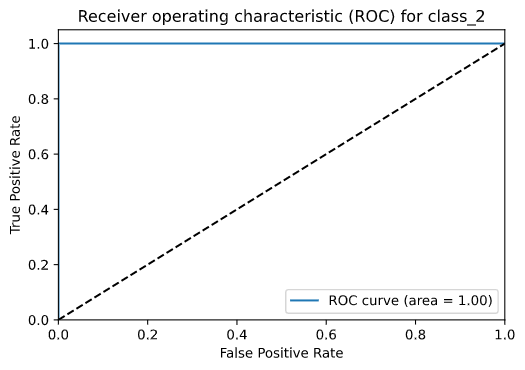
\includegraphics[scale=0.375]{fig/dt_roc2.png}
    \caption{Receiver operating characteristic (ROC) - $class_2$}
    \label{fig:dt_roc2}
    \end{subfigure}
    \vskip\baselineskip
    \begin{subfigure}[b]{0.475\textwidth}
    \centering
    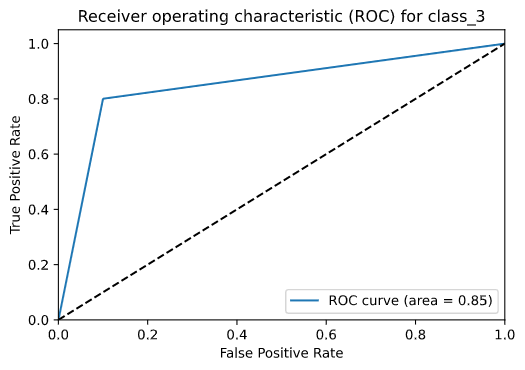
\includegraphics[scale=0.375]{fig/dt_roc3.png}
    \caption{Receiver operating characteristic (ROC) - $class_3$}
    \label{fig:dt_roc3}
    \end{subfigure}
    \hfill
    \begin{subfigure}[b]{0.475\textwidth}
    \centering
    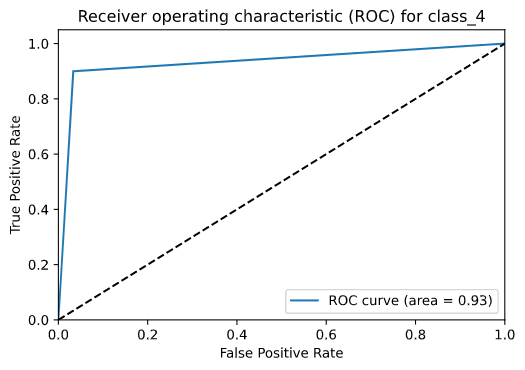
\includegraphics[scale=0.375]{fig/dt_roc4.png}
    \caption{Receiver operating characteristic (ROC) - $class_4$}
    \label{fig:dt_roc4}
    \end{subfigure}
    \caption{Receiver operating characteristic (ROC) para o classificador Árvore de Decisão.}
    \label{dt_roc}
\end{figure}

O valor do coeficiente Kappa para a Árvore de Decisão foi de $0.83$ com as seguintes métricas (Tabela \ref{tab:metrics_dt}).

\begin{verbatim}
 #file: dt.ipynb
 #Kappa
 DT_kappa = cohen_kappa_score(y_true, y_pred_DT)
\end{verbatim}

\begin{table}[H]
\centering
\begin{tabular}{|c|c|c|c|c|}
\hline
\textbf{Métrica}         & \textbf{Class1} & \textbf{Class2} & \textbf{Class3} & \textbf{Class4} \\ \hline
\textbf{Sensibilidade:}  & 1               & 1               & 0.8             & 0.7             \\ \hline
\textbf{True Negative:}  & 1               & 1               & 0.9             & 0.93            \\ \hline
\textbf{Precisão:}       & 1               & 1               & 0.72            & 0.77            \\ \hline
\textbf{Pred. Negativa:} & 1               & 1               & 0.93            & 0.9             \\ \hline
\textbf{False Positive:} & 0               & 0               & 0.1             & 0.06            \\ \hline
\textbf{False Negative:} & 0               & 0.              & 0.2             & 0.3             \\ \hline
\textbf{False Discovery:}    & 0               & 0               & 0.27{]}         & 0.22            \\ \hline
\textbf{Acurácia:}       & 1               & 1               & 0.87            & 0.87            \\ \hline
\end{tabular}
\caption{Métricas - Árvore de Decisão}
\label{tab:metrics_dt}
\end{table}

\newpage
\subsection{Random Forest}

O algoritmo Random Forest é um método \textit{ensemble} que combina a execução de diversas árvores de decisão de maneira que relacione os atributos (características) dos elementos (observações) com seus respectivos rótulos (classes) com uma maior assertividade, diminuindo o efeito de \textit{overfitting} do método árvore de decisão \cite{Igual2017}.

\begin{figure}[H]
 \centering
 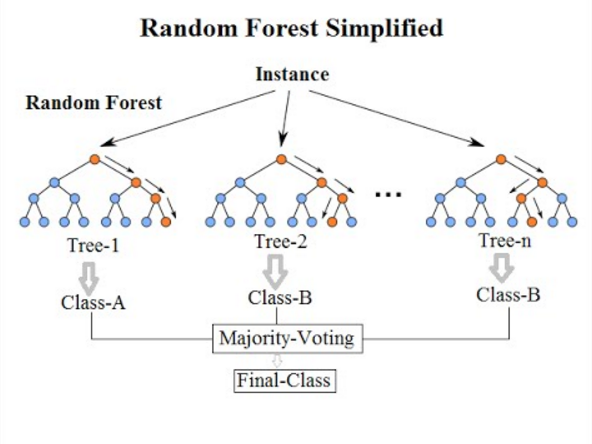
\includegraphics[scale=0.6]{fig/rf_alg.png}
 % scatter.png: 619x604 px, 96dpi, 16.38x15.98 cm, bb=0 0 464 453
 \caption{Exemplo de classificação utilizando Random Forest. Diversas árvores de decisão são executadas simultaneamente, após a execução de todas as $n$ árvores de decisão, através de votação é definida a classe do elemento em análise. Fonte: Venkata Jagannath sob CC BY-SA 3.0}
 \label{fig:rf_alg}
\end{figure}

O algoritmo utilizado está implementado no pacote \verb|sklearn.ensemble| da biblioteca \verb|sklearn| com o seguinte método \verb|RandomForestClassifier|. Os parâmetros utilizados foram os valores default do método, isto é $100$ árvores de decisão por execução e $max\_features=\sqrt{n\_features}$ como o número máximo de características selecionadas para cada árvore de decisão. Além da reamostragem do conjunto de treinamento ser realizada via \textit{bootstrap} com o número máximo de amostras sendo o número de observações do conjunto de treinamento.

\begin{verbatim}
 #file: rf.ipynb
 #Random Forest
 RF = RandomForestClassifier(n_estimators = 100)
 RF.fit(X_train,y_train)
 RF100_res = RF.predict(X_test)
 y_pred_RF100 = np.argmax(RF100_res, axis=1)
 y_predp_RF100 = RF.predict_proba(X_test)
\end{verbatim}


As métricas (Tabela \ref{tab:rf_01}), matriz de confusão (Figura \ref{fig:rf_cm}) e curvas ROC (Figura \ref{rf_roc}) para cada uma das classes são apresentadas abaixo.

\begin{verbatim}
 #file: rf.ipynb
 #Matriz de confusão
 RF100_cm = confusion_matrix(y_true=y_true, 
                             y_pred=y_pred_RF100)
 #Heatmap
 plt.figure(figsize = (10,8))
 ax = plt.axes()
 x_axis_labels = ['class_1', 'class_2', 'class_3', 'class_4'] 
 # labels for x-axis
 y_axis_labels = ['class_1', 'class_2', 'class_3', 'class_4'] 
 # labels for y-axis
 sns.heatmap(RF100_cm,
             vmin=0,
             vmax=10,
             annot=True,
             fmt="d",
             ax = ax,
             xticklabels=x_axis_labels, 
             yticklabels=y_axis_labels)
 ax.set_title('Heatmap for RF100 Classification Model',pad=15)
 #Métricas
 print(classification_report(y_true, y_pred_RF100,
 target_names=class_label))
 print("Accuracy:",metrics.accuracy_score(y_true, y_pred_RF100))
\end{verbatim}


\begin{table}[H]
\centering
\begin{tabular}{c|c|c|c|c|}
\cline{2-5}
                                            & \textbf{precision} & \textbf{recall} & \textbf{f1-score} & \textbf{support} \\ \hline
\multicolumn{1}{|c|}{\textbf{class\_1}}     & 0.91               & 1.00            & 0.95              & 10               \\ \hline
\multicolumn{1}{|c|}{\textbf{class\_2}}     & 1.00               & 0.90            & 0.95              & 10               \\ \hline
\multicolumn{1}{|c|}{\textbf{class\_3}}     & 0.77               & 1.00            & 0.87              & 10               \\ \hline
\multicolumn{1}{|c|}{\textbf{class\_4}}     & 1.00               & 0.70            & 0.82              & 10               \\ \hline
\multicolumn{1}{|c|}{\textbf{accuracy}}     &                    &                 & 0.90              & 40               \\ \hline
\multicolumn{1}{|c|}{\textbf{macro avg}}    & 0.92               & 0.90            & 0.90              & 40               \\ \hline
\multicolumn{1}{|c|}{\textbf{weighted avg}} & 0.92               & 0.90            & 0.90              & 40               \\ \hline
\end{tabular}
\caption{Métricas - Random Forest }
\label{tab:rf_01}
\end{table}

\begin{figure}[H]
 \centering
 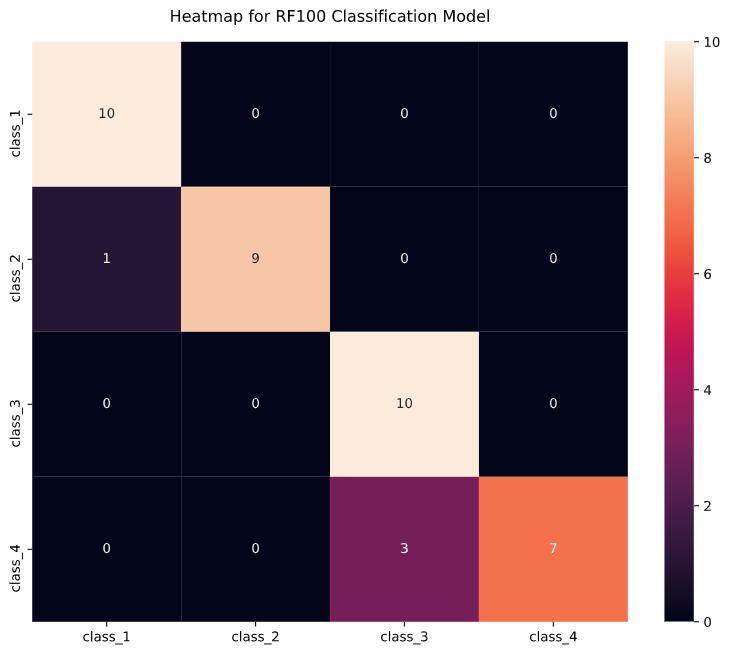
\includegraphics[scale=0.5]{fig/rf_cm.png}
 % scatter.png: 619x604 px, 96dpi, 16.38x15.98 cm, bb=0 0 464 453
 \caption{Matriz de confusão e heatmap para o conjunto de teste - Random Forest.}
 \label{fig:rf_cm}
\end{figure}


\begin{figure}[H]
    \centering
    \begin{subfigure}[b]{0.475\textwidth}
    \centering
    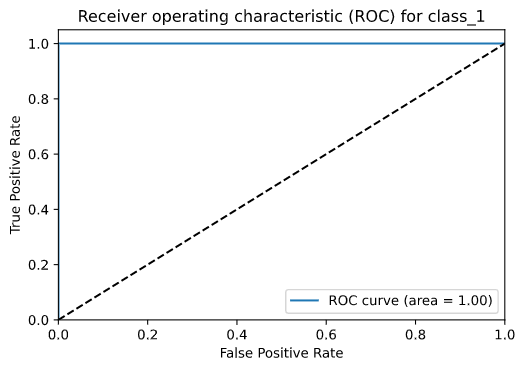
\includegraphics[scale=0.375]{fig/rf_roc1.png}
    \caption{Receiver operating characteristic (ROC) - $class_1$}
    \label{fig:rf_roc1}
    \end{subfigure}
    \hfill
    \begin{subfigure}[b]{0.475\textwidth}
    \centering
    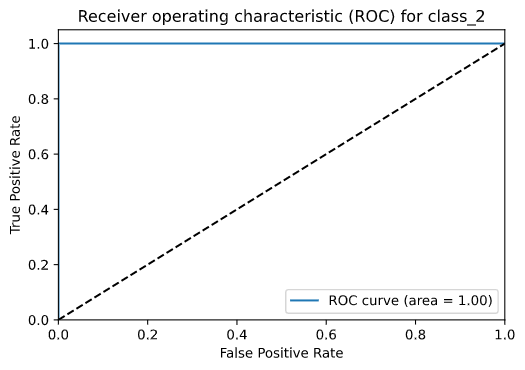
\includegraphics[scale=0.375]{fig/rf_roc2.png}
    \caption{Receiver operating characteristic (ROC) - $class_2$}
    \label{fig:rf_roc2}
    \end{subfigure}
    \vskip\baselineskip
    \begin{subfigure}[b]{0.475\textwidth}
    \centering
    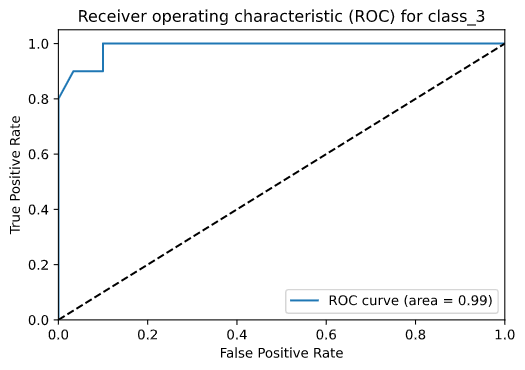
\includegraphics[scale=0.375]{fig/rf_roc3.png}
    \caption{Receiver operating characteristic (ROC) - $class_3$}
    \label{fig:rf_roc3}
    \end{subfigure}
    \hfill
    \begin{subfigure}[b]{0.475\textwidth}
    \centering
    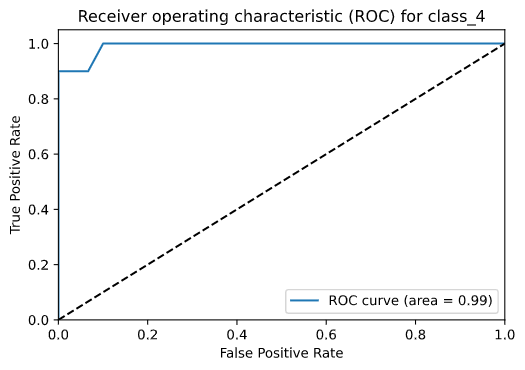
\includegraphics[scale=0.375]{fig/rf_roc4.png}
    \caption{Receiver operating characteristic (ROC) - $class_4$}
    \label{fig:rf_roc4}
    \end{subfigure}
    \caption{Receiver operating characteristic (ROC) para o classificador Random Forest.}
    \label{rf_roc}
\end{figure}

Além das análises apresentadas, foram analisados as características mais relevantes para a classificação, como apresentada na figura \ref{fig:rf_feat}. Essa análise de quais características possuem maior relevância no dataset contribui fornecendo maiores informações a respeito do dataset utilizado.

\begin{figure}[H]
 \centering
 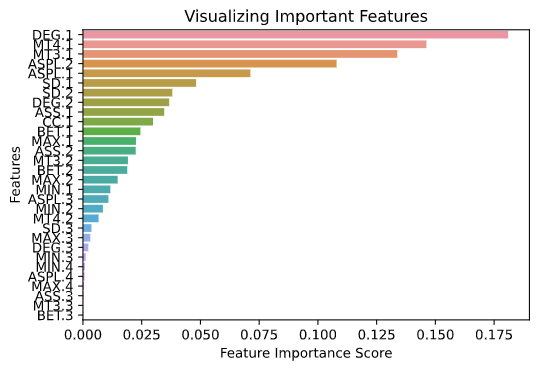
\includegraphics[scale=0.7]{fig/rf_feat.png}
 % scatter.png: 619x604 px, 96dpi, 16.38x15.98 cm, bb=0 0 464 453
 \caption{Características de maior relevância para o classificador Random Forest. A análise pode ser utilizada para unir características semelhantes, selecionando subconjuntos apenas com as características de maior relevância e diminuindo o custo computacional do método.}
 \label{fig:rf_feat}
\end{figure}

O valor do coeficiente Kappa para o classificador Random Forest foi de $0.86$ com as seguintes métricas (\ref{tab:metrics_rf}):

\begin{table}[H]
\centering
\begin{tabular}{|c|l|l|l|l|}
\hline
\textbf{Métrica}         & \textbf{Class1} & \textbf{Class2} & \textbf{Class3} & \textbf{Class4} \\ \hline
\textbf{Sensibilidade:}  & 1               & 0.9             & 1               & 0.7             \\ \hline
\textbf{True Negative:}  & 0.96            & 1               & 0.9             & 1               \\ \hline
\textbf{Precisão:}       & 0.90            & 1               & 0.76            & 1               \\ \hline
\textbf{Pred. Negativa:} & 1               & 0.96            & 1               & 0.9             \\ \hline
\textbf{False Positive:} & 0.03            & 0               & 0.1             & 0               \\ \hline
\textbf{False Negative:} & 0               & 0.1             & 0               & 0.3             \\ \hline
\textbf{F Discovery:}    & 0.09            & 0               & 0.23            & 0               \\ \hline
\textbf{Acurácia:}       & 0.97            & 0.97            & 0.92            & 0.92            \\ \hline
\end{tabular}
\caption{Métricas - Random Forest}
\label{tab:metrics_rf}
\end{table}

\subsection{Gradient Boosting}

Um outro método do tipo \textit{ensemble} proposto é o Gradient Boosting inicialmente apresentaado por \cite{Friedman2000}. Utilizando a teoria \textit{boosting} com ferramental matemático (otimização) e estatístico o método Gradient Boosting realiza uma busca do ponto mínimo da função \textit{loss} associada ao modelo.

Em outras palavras, busca-se associar um funcional desconhecido utilizando um conjunto $(x,y)_{i=1}^N$, onde  $x$ são as características das observações e $y$ os rótulos de cada observação \cite{Natekin2013}. Dessa forma busca-se definir um funcional $\hat{f}$ de tal forma que $x \xrightarrow{f} y$ seja aproximado por $\hat{f}$ minimizando uma função $\Psi(y,f)$:
\begin{equation}
 \hat{f}(x) = y
\end{equation}
\begin{equation}
\label{gb_eq}
 \hat{f}(x) = \underset{f(x)}{\mathrm{argmin}}\Psi(y,f(x))
\end{equation}

A equação \ref{gb_eq} é reescrita de maneira a obter a função objetiva que sera diferenciada e utilizando a técnica de otimização do gradiente descendente busca-se definir o seu ponto de mínimo. O método pode ser detalhado em \cite{Natekin2013}.

O algoritmo utilizado está implementado no pacote \verb|sklearn.ensemble| da biblioteca \verb|sklearn| com o seguinte método \verb|GradientBoostingClassifier|. 

O método possuí diversos parâmetros e como o objetivo deste relatório não é refinar métodos de machine learning optou-se por analisar somente um parâmetro do método Gradient Boosting, contudo é válido reforçar que pode-se utilizar de diversas outras abordagens para obter melhores valores nas métricas de avaliação, como por exemplo uma busca em \textit{grid} de diversos parâmetros e valores.

\begin{verbatim}
 #file:grad_boost.ipynb
 #Taxas de aprendizagem
 lr_list = [0.05, 0.075, 0.1, 0.25, 0.5, 0.75, 1]
 for learning_rate in lr_list:
    gb_clf = OneVsRestClassifier(GradientBoostingClassifier(n_estimators=100,                                                            learning_rate=learning_rate, max_features=None, max_depth=3, random_state=None))
    gb_fit = gb_clf.fit(X_train, y_train)
    print("Learning rate: ", learning_rate)
    print("Accuracy score (training): {0:.3f}".format(gb_fit.score(X_train,
    y_train)))
    print("Accuracy score (teste): {0:.3f}".format(gb_fit.score(X_test,
    y_test)))  
\end{verbatim}

O parâmetro analisado foi a taxa de aprendizagem do algoritmo, com os seguintes valores: $0.05, 0.075, 0.1, 0.25, 0.5, 0.75$ e $1$. Os demais parâmetros foram considerados os valores \textit{default} do método. A execução das taxas de aprendizagem resultou em valores de acurácia diversos 
\footnote{Os demais valores estão no arquivo grad\_boost.ipynb.}, a maior taxa de acurácia foi obtida com a taxa de $0.5$, a qual foi utilizada ao decorrer das análises. 

\begin{verbatim}
 #file: grad_boost.ipynb
 #L.R. 0.5
 gb_clf = OneVsRestClassifier(GradientBoostingClassifier(n_estimators=100,                                                        learning_rate=0.5, max_features=None, max_depth=3, random_state=None))
 y_predp_ovr_gb = gb_clf.fit(X_train, y_train).predict_proba(X_test)
 y_pred_ovr_gb = gb_clf.fit(X_train, y_train).predict(X_test)
 y_pred_gb = np.argmax(y_pred_ovr_gb, axis=1)
\end{verbatim}

As métricas (Tabela \ref{tab:gb_01}), matriz de confusão (Figura \ref{fig:gb_cm}) e curvas ROC (Figura \ref{gb_roc}) para cada uma das classes foram as seguintes:

\begin{verbatim}
 #file: grad_boost.ipynb
 #Matriz de confusão
 gb_cm = confusion_matrix(y_true=y_true, 
                         y_pred=y_pred_gb)
 #Heatmap
 plt.figure(figsize = (10,8))
 ax = plt.axes()
 x_axis_labels = ['class_1', 'class_2', 'class_3', 'class_4'] 
 # labels for x-axis
 y_axis_labels = ['class_1', 'class_2', 'class_3', 'class_4'] 
 # labels for y-axis
 sns.heatmap(gb_cm,
             vmin=0,
             vmax=10,
             annot=True,
             fmt="d",
             ax = ax,
             xticklabels=x_axis_labels, 
             yticklabels=y_axis_labels)
 ax.set_title('Heatmap for Gradient Boosting Classification Model',pad=15)
 print(classification_report(y_true, y_pred_gb, target_names=class_label))
 print("Accuracy:",metrics.accuracy_score(y_true, y_pred_gb))
\end{verbatim}


\newpage
\begin{table}[H]
\centering
\begin{tabular}{c|c|c|c|c|}
\cline{2-5}
                                            & \textbf{precision} & \textbf{recall} & \textbf{f1-score} & \textbf{support} \\ \hline
\multicolumn{1}{|c|}{\textbf{class\_1}}     & 1.00               & 0.80            & 0.89              & 10               \\ \hline
\multicolumn{1}{|c|}{\textbf{class\_2}}     & 1.00               & 1.00            & 1.00              & 10               \\ \hline
\multicolumn{1}{|c|}{\textbf{class\_3}}     & 0.77               & 1.00            & 0.87              & 10               \\ \hline
\multicolumn{1}{|c|}{\textbf{class\_4}}     & 1.00               & 0.90            & 0.95              & 10               \\ \hline
\multicolumn{1}{|c|}{\textbf{accuracy}}     &                    &                 & 0.93              & 40               \\ \hline
\multicolumn{1}{|c|}{\textbf{macro avg}}    & 0.94               & 0.92            & 0.93              & 40               \\ \hline
\multicolumn{1}{|c|}{\textbf{weighted avg}} & 0.94               & 0.93            & 0.93              & 40               \\ \hline
\end{tabular}
\caption{Métricas - Gradient Boosting - L.R: $0.5$}
\label{tab:gb_01}
\end{table}


\begin{figure}[H]
 \centering
 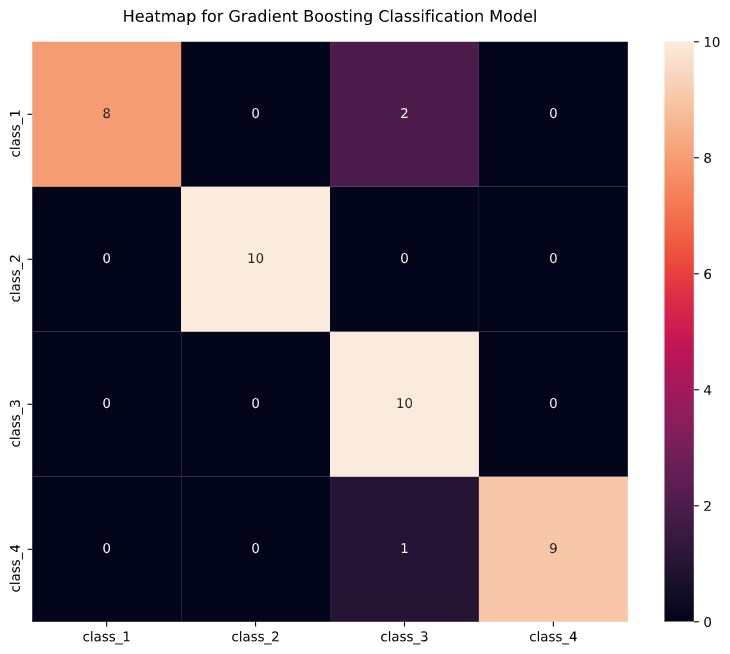
\includegraphics[scale=0.5]{fig/gb_cm.png}
 % scatter.png: 619x604 px, 96dpi, 16.38x15.98 cm, bb=0 0 464 453
 \caption{Matriz de confusão e heatmap para o conjunto de teste - Gradient Boosting L.R. :$0.5$.}
 \label{fig:gb_cm}
\end{figure}



\begin{figure}[H]
    \centering
    \begin{subfigure}[b]{0.475\textwidth}
    \centering
    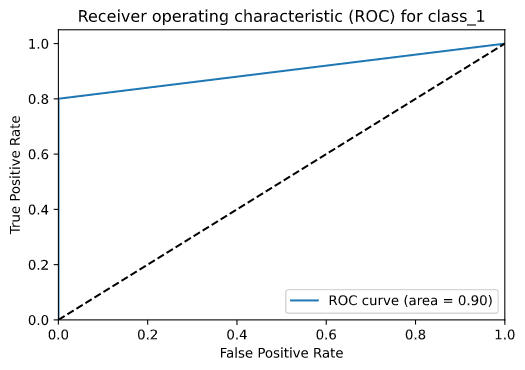
\includegraphics[scale=0.375]{fig/gb_roc1.png}
    \caption{Receiver operating characteristic (ROC) - $class_1$}
    \label{fig:gb_roc1}
    \end{subfigure}
    \hfill
    \begin{subfigure}[b]{0.475\textwidth}
    \centering
    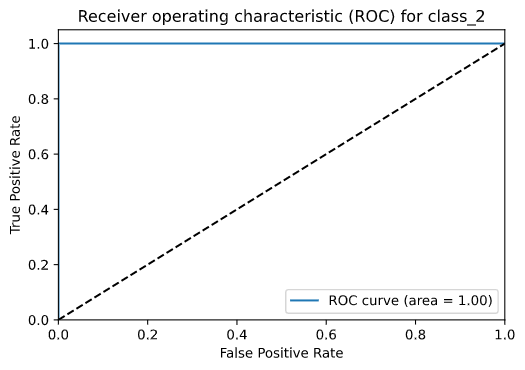
\includegraphics[scale=0.375]{fig/gb_roc2.png}
    \caption{Receiver operating characteristic (ROC) - $class_2$}
    \label{fig:gb_roc2}
    \end{subfigure}
    \vskip\baselineskip
    \begin{subfigure}[b]{0.475\textwidth}
    \centering
    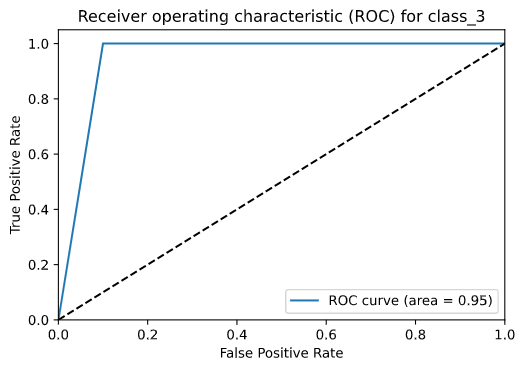
\includegraphics[scale=0.375]{fig/gb_roc3.png}
    \caption{Receiver operating characteristic (ROC) - $class_3$}
    \label{fig:gb_roc3}
    \end{subfigure}
    \hfill
    \begin{subfigure}[b]{0.475\textwidth}
    \centering
    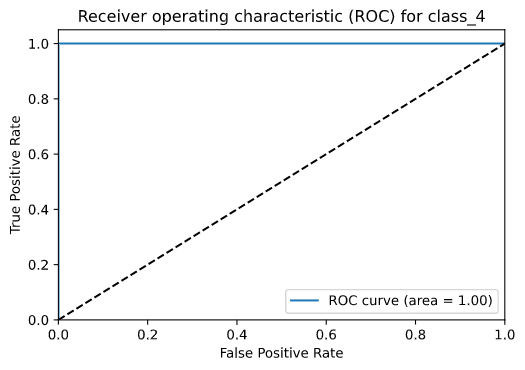
\includegraphics[scale=0.375]{fig/gb_roc4.png}
    \caption{Receiver operating characteristic (ROC) - $class_4$}
    \label{fig:gb_roc4}
    \end{subfigure}
    \caption{Receiver operating characteristic (ROC) para o classificador Grandient Boosting.}
    \label{gb_roc}
\end{figure}


O valor do coeficiente Kappa para o classificador Gradient Boosting foi de $0.9$ com as seguintes métricas (\ref{tab:metrics_gb}):

\begin{table}[H]
\centering
\begin{tabular}{|c|c|c|c|c|}
\hline
\textbf{Métricas}        & \textbf{Class1} & \textbf{Class2} & \textbf{Class3} & \textbf{Class4} \\ \hline
\textbf{Sensibilidade:}  & 0.8             & 1               & 1               & 0.9             \\ \hline
\textbf{True Negative:}  & 1               & 1               & 0.9             & 1               \\ \hline
\textbf{Precisão:}       & 1               & 1               & 0.76            & 1               \\ \hline
\textbf{Pred. Negativa:} & 0.93            & 1               & 1               & 0.96            \\ \hline
\textbf{False Positive:} & 0               & 0               & 0.1             & 0               \\ \hline
\textbf{False Negative:} & 0.2             & 0               & 0               & 0.1             \\ \hline
\textbf{F Discovery:}    & 0               & 0               & 0.23            & 0               \\ \hline
\textbf{Acurácia:}       & 0.95            & 1               & 0.92            & 0.97            \\ \hline
\end{tabular}
\caption{Métricas - Gradiente Boosting - L.R.:$0.5$}
\label{tab:metrics_gb}
\end{table}

\newpage
\subsection{XGBoost}


Proposto inicialmente por \cite{Chen2016} o método XGBoost também utiliza metodologia análoga aos métodos anteriores, isto é, é um método do tipo \textit{boosting} que busca minimizar uma função \textit{loss}. Quando comparado com outros métodos XGBoost possui recursos que aumentam sua acurácia dependendo do dataset utilizado. Maiores informações sobre o método e a abordagem matemática por ser acessada em \cite{Chen2016}.

O algoritmo utilizado está implementado na biblioteca \verb|xgboost| com o seguinte método \verb|XGBClassifier|. 

O método possuí diversos parâmetros, como o objetivo deste relatório não é refinar métodos de machine learning optou-se por analisar somente um parâmetro do método XGBoost, contudo é válido reforçar que pode-se utilizar de diversas outras abordagens para obter melhores valores nas métricas de avaliação, como por exemplo uma busca em \textit{grid} de diversos parâmetros e valores.

O parâmetro analisado foi a taxa de aprendizagem do algoritmo, analisando os seguintes valores: $0.05, 0.075, 0.1, 0.25, 0.5, 0.75$ e $1$. Os demais parâmetros foram considerados os valores default. A execução das taxas de aprendizagem resultou em valores de acurácia diversos 
\footnote{Os demais valores estão no arquivo XGBoost.ipynb.}, a maior taxa de acurácia foi obtida com a taxa de $0.075$, a qual foi utilizada ao decorrer das análises. 

\begin{verbatim}
 #file:XGBoost.ipynb
 #Analisando LR
 lr_list = [0.05, 0.075, 0.1, 0.25, 0.5, 0.75, 1]
 for learning_rate in lr_list:
    xgb_clf = OneVsRestClassifier(XGBClassifier(eval_metric='mlogloss',
                                                use_label_encoder=False,
                                                learning_rate=learning_rate)
                                                )

    xgb_fit = xgb_clf.fit(X_train, y_train)
    print("Learning rate: ", learning_rate)
    print("Accuracy score (training): {0:.3f}".format(xgb_fit.score(X_train,
    y_train)))
    print("Accuracy score (teste): {0:.3f}".format(xgb_fit.score(X_test,
    y_test)))
 #LR
 xgb_clf = OneVsRestClassifier(XGBClassifier(eval_metric='mlogloss',
                                                 use_label_encoder=False,
                                                 learning_rate=0.075))
 y_predp_ovr_xgb = xgb_clf.fit(X_train, y_train).predict_proba(X_test)
 y_pred_ovr_xgb = xgb_clf.fit(X_train, y_train).predict(X_test)
 y_pred_xgb = np.argmax(y_pred_ovr_xgb, axis=1)
\end{verbatim}


As métricas (Tabela \ref{tab:xgb_01}), matriz de confusão (Figura \ref{fig:xgb_cm}) e curvas ROC (Figura \ref{xgb_roc}) para cada uma das classes foram as seguintes:

\begin{verbatim}
 #file: XGBoost.ipynb
 #Matriz de confusão
 xgb_cm = confusion_matrix(y_true=y_true, 
                           y_pred=y_pred_xgb)
 #Heatmap
 plt.figure(figsize = (10,8))
 ax = plt.axes()
 x_axis_labels = ['class_1', 'class_2', 'class_3', 'class_4'] # labels for x-axis
 y_axis_labels = ['class_1', 'class_2', 'class_3', 'class_4'] # labels for y-axis
 sns.heatmap(xgb_cm,
             vmin=0,
             vmax=10,
             annot=True,
             fmt="d",
             ax = ax,
             xticklabels=x_axis_labels, 
             yticklabels=y_axis_labels)
 ax.set_title('Heatmap for X Gradient Boosting Classification Model',pad=15)
 #Métricas
 print(classification_report(y_true, y_pred_xgb, target_names=class_label))
 print("Accuracy:",metrics.accuracy_score(y_true, y_pred_xgb))
 \end{verbatim}

\newpage
\begin{table}[H]
\centering
\begin{tabular}{l|l|l|l|l|}
\cline{2-5}
                                            & \textbf{precision} & \textbf{recall} & \textbf{f1-score} & \textbf{support} \\ \hline
\multicolumn{1}{|l|}{\textbf{class\_1}}     & 0.83               & 1.00            & 0.91              & 10               \\ \hline
\multicolumn{1}{|l|}{\textbf{class\_2}}     & 1.00               & 1.00            & 1.00              & 10               \\ \hline
\multicolumn{1}{|l|}{\textbf{class\_3}}     & 0.88               & 0.70            & 0.78              & 10               \\ \hline
\multicolumn{1}{|l|}{\textbf{class\_4}}     & 0.90               & 0.90            & 0.90              & 10               \\ \hline
\multicolumn{1}{|l|}{\textbf{accuracy}}     &                    &                 & 0.90              & 40               \\ \hline
\multicolumn{1}{|l|}{\textbf{macro avg}}    & 0.90               & 0.90            & 0.90              & 40               \\ \hline
\multicolumn{1}{|l|}{\textbf{weighted avg}} & 0.90               & 0.90            & 0.90              & 40               \\ \hline
\end{tabular}
\caption{Métricas - XGBoost - L.R: $0.075$}
\label{tab:xgb_01}
\end{table}


\begin{figure}[H]
 \centering
 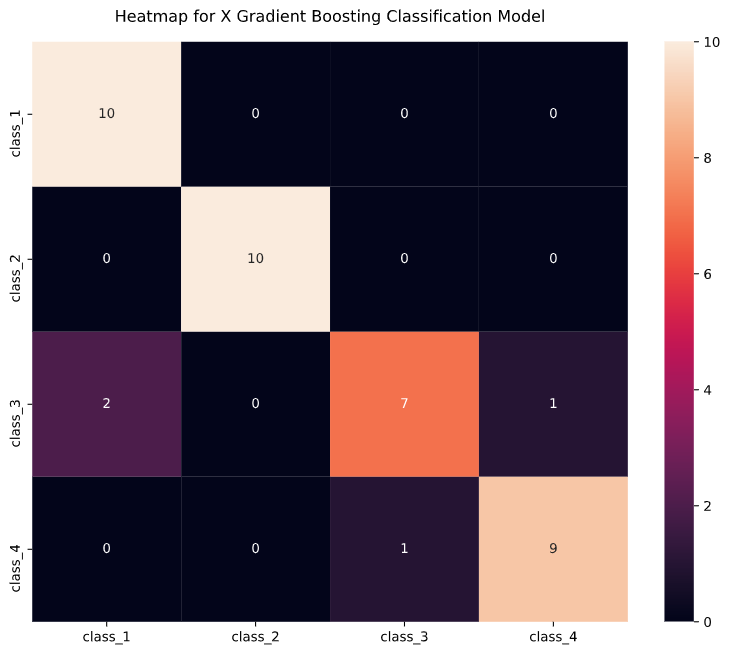
\includegraphics[scale=0.5]{fig/xgb_cm.png}
 % scatter.png: 619x604 px, 96dpi, 16.38x15.98 cm, bb=0 0 464 453
 \caption{Matriz de confusão e heatmap para o conjunto de teste - XGBoost L.R. :$0.075$.}
 \label{fig:xgb_cm}
\end{figure}


\begin{figure}
    \centering
    \begin{subfigure}[b]{0.475\textwidth}
    \centering
    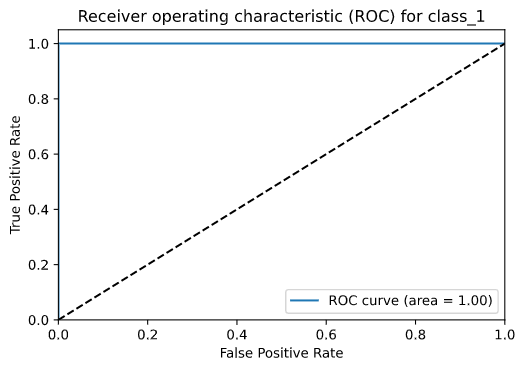
\includegraphics[scale=0.375]{fig/xgb_roc1.png}
    \caption{Receiver operating characteristic (ROC) - $class_1$}
    \label{fig:xgb_roc1}
    \end{subfigure}
    \hfill
    \begin{subfigure}[b]{0.475\textwidth}
    \centering
    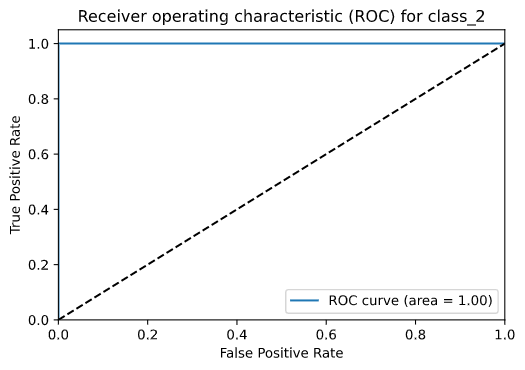
\includegraphics[scale=0.375]{fig/xgb_roc2.png}
    \caption{Receiver operating characteristic (ROC) - $class_2$}
    \label{fig:xgb_roc2}
    \end{subfigure}
    \vskip\baselineskip
    \begin{subfigure}[b]{0.475\textwidth}
    \centering
    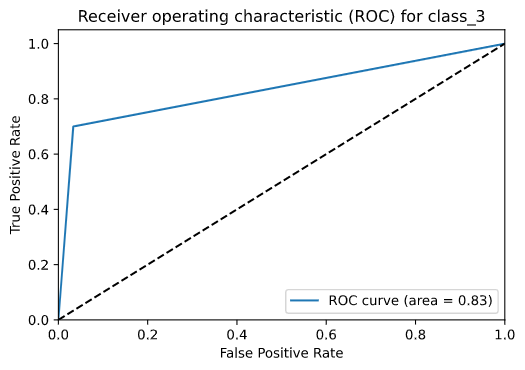
\includegraphics[scale=0.375]{fig/xgb_roc3.png}
    \caption{Receiver operating characteristic (ROC) - $class_3$}
    \label{fig:xgb_roc3}
    \end{subfigure}
    \hfill
    \begin{subfigure}[b]{0.475\textwidth}
    \centering
    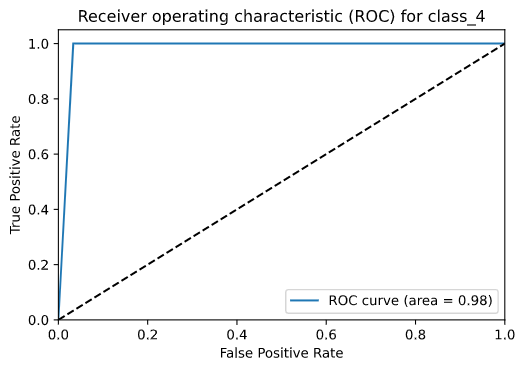
\includegraphics[scale=0.375]{fig/xgb_roc4.png}
    \caption{Receiver operating characteristic (ROC) - $class_4$}
    \label{fig:xgb_roc4}
    \end{subfigure}
    \caption{Receiver operating characteristic (ROC) para o classificador XGBoost.}
    \label{xgb_roc}
\end{figure}

O valor do coeficiente Kappa para o classificador XGBoost foi de $0.86$ com as seguintes métricas (\ref{tab:metrics_xgb}):

\begin{table}[H]
\centering
\begin{tabular}{|c|c|c|c|c|}
\hline
\textbf{Métrica}         & \textbf{Class1} & \textbf{Class2} & \textbf{Class3} & \textbf{Class4} \\ \hline
\textbf{Sensibilidade:}  & 1               & 1               & 0.7             & 0.9             \\ \hline
\textbf{True Negative:}  & 0.93            & 1               & 0.96            & 0.96            \\ \hline
\textbf{Precisão:}       & 0.83            & 1               & 0.87            & 0.9             \\ \hline
\textbf{Pred. Negativa:} & 1               & 1               & 0.9             & 0.96            \\ \hline
\textbf{False Positive:} & 0.06            & 0               & 0.03            & 0.03            \\ \hline
\textbf{False Negative:} & 0               & 0               & 0.3             & 0.1             \\ \hline
\textbf{F Discovery:}    & 0.16            & 0               & 0.125           & 0.1             \\ \hline
\textbf{Acurácia:}       & 0.95            & 1               & 0.9             & 0.95            \\ \hline
\end{tabular}
\caption{Métricas - XGBoost - L.R.:$0.075$}
\label{tab:metrics_xgb}
\end{table}

\newpage
\subsection{Support Vector Machine (SVM)}

O objetivo de uma máquina de vetor suporte (do inglês Support Vector Machine (SVM)) é definir um hiperplano em um espaço $n-$dimensional de maneira que divida os pontos em classes, detalhes e demonstrações matemáticas para SVM podem ser encontradas em \cite{bishop:2006:PRML, Smola04atutorial}.

\begin{figure}[H]
 \centering
 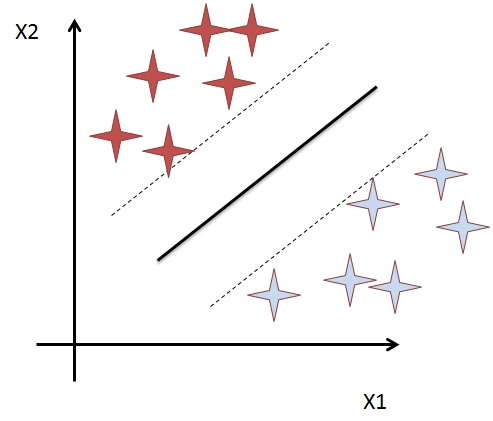
\includegraphics[scale=0.6]{fig/svm_alg.jpg}
 % scatter.png: 619x604 px, 96dpi, 16.38x15.98 cm, bb=0 0 464 453
 \caption{Exemplo de classificação utilizando SVM.  Fonte: Roni Shouval sob CC BY-SA 3.0}
 \label{fig:svm_alg}
\end{figure}

O algoritmo utilizado está implementado no pacote \verb|svm| da biblioteca \verb|sklearn| com o seguinte método \verb|SVC|. 

O método possui diversos parâmetros, como o objetivo deste relatório não é refinar métodos de machine learning optou-se por analisar somente um parâmetro do método SVM, contudo é válido reforçar que pode-se utilizar de diversas outras abordagens para obter melhores valores nas métricas de avaliação, como por exemplo uma busca em grid de diversos parâmetros e valores.

O parâmetro analisado foi a função kernel do algoritmo, analisando o comportamento do método com seguintes kernels: \verb|'linear', 'poly', 'rbf', 'sigmoid'|. Os demais parâmetros foram considerados os valores default. A execução com diversas funções kernel resultou em valores de acurácia diversos 
\footnote{Os demais valores estão no arquivo svm.ipynb.}, a maior taxa de acurácia foi obtida com o kernel linear, o qual foi utilizado ao decorrer das análises. 

\begin{verbatim}
 #file: svm.ipynb
 krnl = ['linear', 'poly', 'rbf', 'sigmoid']
 for kernel in krnl:
    svm_clf = OneVsRestClassifier(svm.SVC(kernel=kernel,
                                          probability=True))

    svm_fit = svm_clf.fit(X_train, y_train)

    print("Learning rate: ", kernel)
    print("Accuracy score (training): {0:.3f}".format(svm_fit.score(X_train,
    y_train)))
    print("Accuracy score (teste): {0:.3f}".format(svm_fit.score(X_test,
    y_test)))
\end{verbatim}

As métricas (Tabela \ref{tab:svm_01}), matriz de confusão (Figura \ref{fig:svm_cm}) e curvas ROC (Figura \ref{svm_roc}) para cada uma das classes foram as seguintes:

\begin{verbatim}
 #file: svm.ipynb
 svm_clf = OneVsRestClassifier(svm.SVC(kernel='linear',
                                      probability=True))

 y_predp_ovr_svm = svm_clf.fit(X_train, y_train).predict_proba(X_test)
 y_pred_ovr_svm = svm_clf.fit(X_train, y_train).predict(X_test)
 y_pred_svm = np.argmax(y_pred_ovr_svm, axis=1)
 #Matriz de confusão
 svm_cm = confusion_matrix(y_true=y_true, 
                          y_pred=y_pred_svm)
 #Heatmap
 plt.figure(figsize = (10,8))
 ax = plt.axes()
 x_axis_labels = ['class_1', 'class_2', 'class_3', 'class_4'] 
 # labels for x-axis
 y_axis_labels = ['class_1', 'class_2', 'class_3', 'class_4'] 
 # labels for y-axis
 sns.heatmap(svm_cm,
             vmin=0,
             vmax=10,
             annot=True,
             fmt="d",
             ax = ax,
             xticklabels=x_axis_labels, 
             yticklabels=y_axis_labels)
 ax.set_title('Heatmap for Gradient Boosting Classification Model',pad=15)
 print(classification_report(y_true, y_pred_svm, target_names=class_label))
 print("Accuracy:",metrics.accuracy_score(y_true, y_pred_svm))
\end{verbatim}


\begin{table}[H]
\centering
\begin{tabular}{c|c|c|c|c|}
\cline{2-5}
                                            & \textbf{precision} & \textbf{recall} & \textbf{f1-score} & \textbf{support} \\ \hline
\multicolumn{1}{|c|}{\textbf{class\_1}}     & 0.59               & 1.00            & 0.74              & 10               \\ \hline
\multicolumn{1}{|c|}{\textbf{class\_2}}     & 1.00               & 1.00            & 1.00              & 10               \\ \hline
\multicolumn{1}{|c|}{\textbf{class\_3}}     & 0.67               & 0.20            & 0.31              & 10               \\ \hline
\multicolumn{1}{|c|}{\textbf{class\_4}}     & 0.90               & 0.90            & 0.90              & 10               \\ \hline
\multicolumn{1}{|c|}{\textbf{accuracy}}     &                    &                 & 0.78              & 40               \\ \hline
\multicolumn{1}{|c|}{\textbf{macro avg}}    & 0.79               & 0.78            & 0.74              & 40               \\ \hline
\multicolumn{1}{|c|}{\textbf{weighted avg}} & 0.79               & 0.78            & 0.74              & 40               \\ \hline
\end{tabular}
\caption{Métricas - SVM Linear}
\label{tab:svm_01}
\end{table}


\begin{figure}[H]
 \centering
 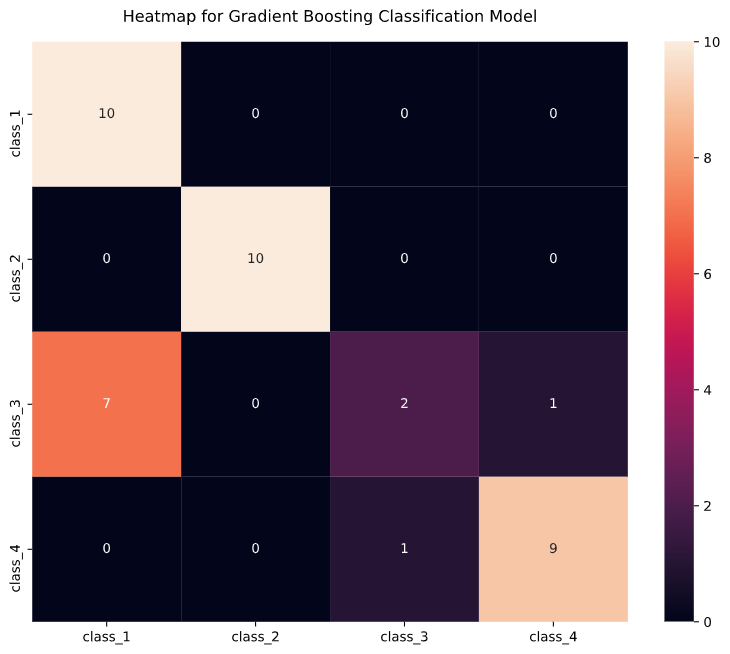
\includegraphics[scale=0.5]{fig/svm_cm.png}
 % scatter.png: 619x604 px, 96dpi, 16.38x15.98 cm, bb=0 0 464 453
 \caption{Matriz de confusão e heatmap para o conjunto de teste - SVM Linear.}
 \label{fig:svm_cm}
\end{figure}

\begin{figure}[H]
    \centering
    \begin{subfigure}[b]{0.475\textwidth}
    \centering
    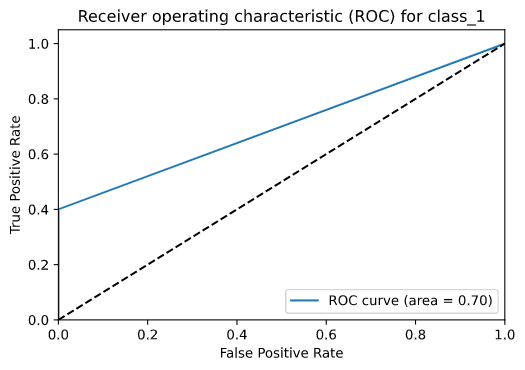
\includegraphics[scale=0.375]{fig/svm_roc1.png}
    \caption{Receiver operating characteristic (ROC) - $class_1$}
    \label{fig:svm_roc1}
    \end{subfigure}
    \hfill
    \begin{subfigure}[b]{0.475\textwidth}
    \centering
    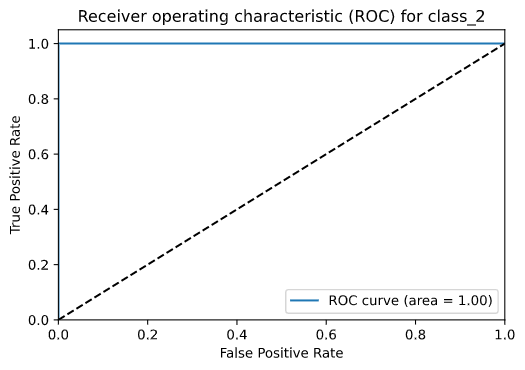
\includegraphics[scale=0.375]{fig/svm_roc2.png}
    \caption{Receiver operating characteristic (ROC) - $class_2$}
    \label{fig:svm_roc2}
    \end{subfigure}
    \vskip\baselineskip
    \begin{subfigure}[b]{0.475\textwidth}
    \centering
    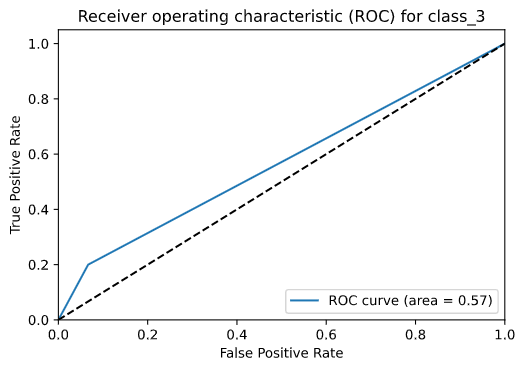
\includegraphics[scale=0.375]{fig/svm_roc3.png}
    \caption{Receiver operating characteristic (ROC) - $class_3$}
    \label{fig:svm_roc3}
    \end{subfigure}
    \hfill
    \begin{subfigure}[b]{0.475\textwidth}
    \centering
    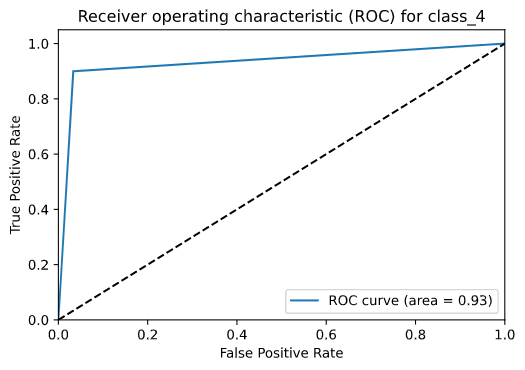
\includegraphics[scale=0.375]{fig/svm_roc4.png}
    \caption{Receiver operating characteristic (ROC) - $class_4$}
    \label{fig:svm_roc4}
    \end{subfigure}
    \caption{Receiver operating characteristic (ROC) para o classificador SVM Linear.}
    \label{svm_roc}
\end{figure}

O valor do coeficiente Kappa para o classificador Gradient Boosting foi de $0.7$ com as seguintes métricas (\ref{tab:metrics_svm}):

\begin{table}[H]
\centering
\begin{tabular}{|c|c|c|c|c|}
\hline
\textbf{Métricas}        & \textbf{Class1} & \textbf{Class2} & \textbf{Class3} & \textbf{Class4} \\ \hline
\textbf{Sensibilidade:}  & 1               & 1               & 0.2             & 0.9             \\ \hline
\textbf{True Negative:}  & 0.76            & 1               & 0.96            & 0.96            \\ \hline
\textbf{Precisão:}       & 0.58            & 1               & 0.66            & 0.9             \\ \hline
\textbf{Pred. Negativa:} & 1               & 1               & 0.78            & 0.96            \\ \hline
\textbf{False Positive:} & 0.2             & 0               & 0.03            & 0.03            \\ \hline
\textbf{False Negative:} & 0               & 0               & 0.8             & 0.1             \\ \hline
\textbf{F Discovery:}    & 0.41            & 0               & 0.33            & 0.1             \\ \hline
\textbf{Acurácia:}       & 0.82            & 1               & 0.77            & 0.95            \\ \hline
\end{tabular}
\caption{Métricas - SVM Linear}
\label{tab:metrics_svm}
\end{table}


\newpage
\section{Conclusão}

A execução de diversos métodos de aprendizagem de máquina proporcionou uma avaliação do comportamento ao dataset escolhido. Inicialmente foi realizado uma curva ROC para os métodos (Figura \ref{roc}):

\begin{verbatim}
 #file: comparison.ipynb
 for i in range(class_label.shape[0]):
    plt.figure(figsize = (10,6))
    plt.plot(fpr_svm[i], 
             tpr_svm[i],
             color='red', 
             label='ROC curve for SVM (area = %0.2f)' % roc_auc_svm[i])
    plt.plot(fpr_xgb[i], 
             tpr_xgb[i],
             color='black', 
             label='ROC curve for XGBoost (area = %0.2f)' % roc_auc_xgb[i])
    plt.plot(fpr_RF100[i], 
             tpr_RF100[i],
             color='green', 
             label='ROC curve for RF100 (area = %0.2f)' % roc_auc_RF100[i])
    plt.plot(fpr_KNN1[i], 
             tpr_KNN1[i],
             color='blue', 
             label='ROC curve for KNN (area = %0.2f)' % roc_auc_KNN1[i])
    plt.plot(fpr_gb[i], 
             tpr_gb[i],
             color='cyan', 
             label='ROC curve for Gradient Boosting (area = %0.2f)' % roc_auc_gb[i])
    plt.plot(fpr_DT[i], 
             tpr_DT[i],
             color='magenta', 
             label='ROC curve for DT (area = %0.2f)' % roc_auc_DT[i])
    plt.plot([0, 1], [0, 1], 'k--')
    plt.xlim([0.0, 1.0])
    plt.ylim([0.0, 1.05])
    plt.xlabel('False Positive Rate')
    plt.ylabel('True Positive Rate')
    plt.title('Receiver operating characteristic (ROC) for %s' % class_label[i])
    plt.legend(loc="lower right")
    plt.show()
\end{verbatim}


\begin{figure}[H]
    \centering
    \begin{subfigure}[b]{0.475\textwidth}
    \centering
    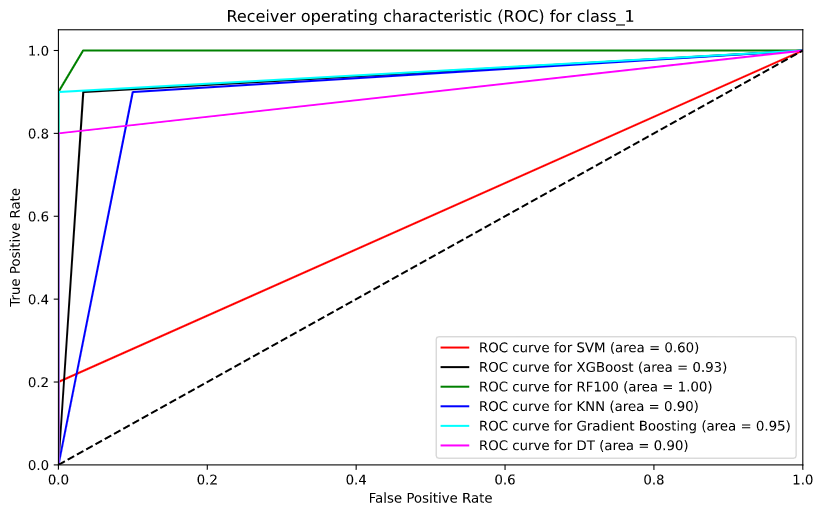
\includegraphics[scale=0.25]{fig/roc1.png}
    \caption{Receiver operating characteristic (ROC) - $class_1$}
    \label{fig:roc1}
    \end{subfigure}
    \hfill
    \begin{subfigure}[b]{0.475\textwidth}
    \centering
    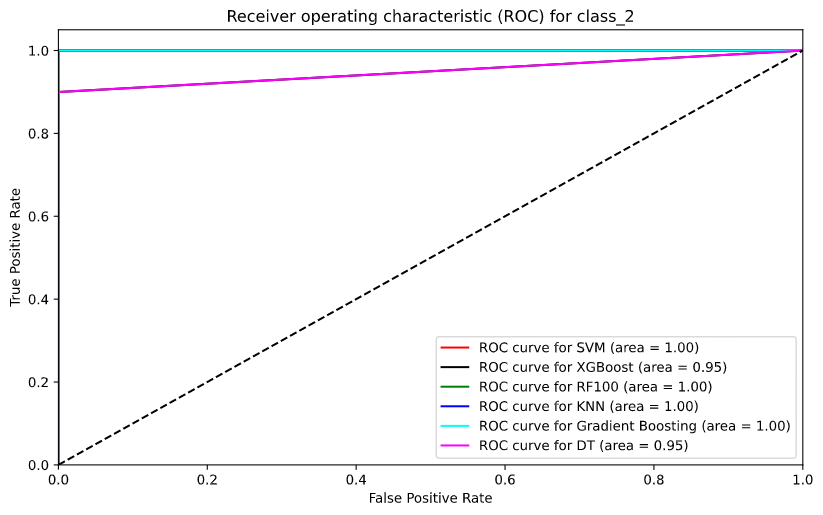
\includegraphics[scale=0.25]{fig/roc2.png}
    \caption{Receiver operating characteristic (ROC) - $class_2$}
    \label{fig:roc2}
    \end{subfigure}
    \vskip\baselineskip
    \begin{subfigure}[b]{0.475\textwidth}
    \centering
    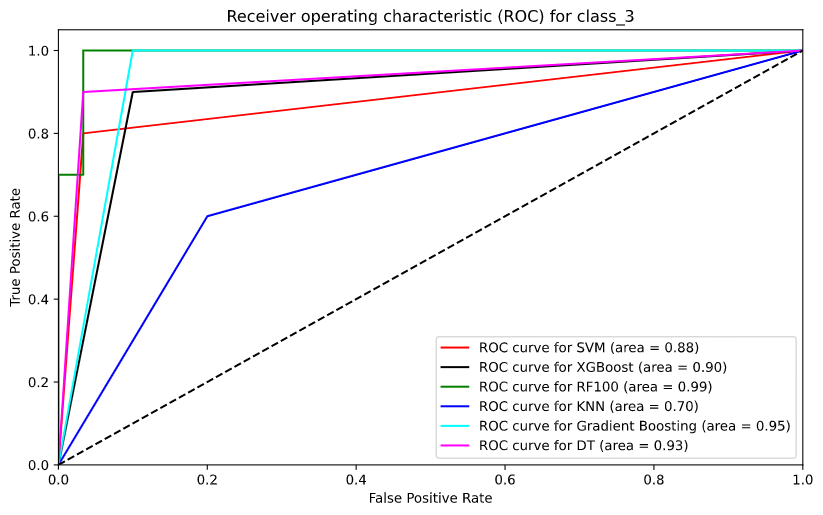
\includegraphics[scale=0.25]{fig/roc3.png}
    \caption{Receiver operating characteristic (ROC) - $class_3$}
    \label{fig:roc3}
    \end{subfigure}
    \hfill
    \begin{subfigure}[b]{0.475\textwidth}
    \centering
    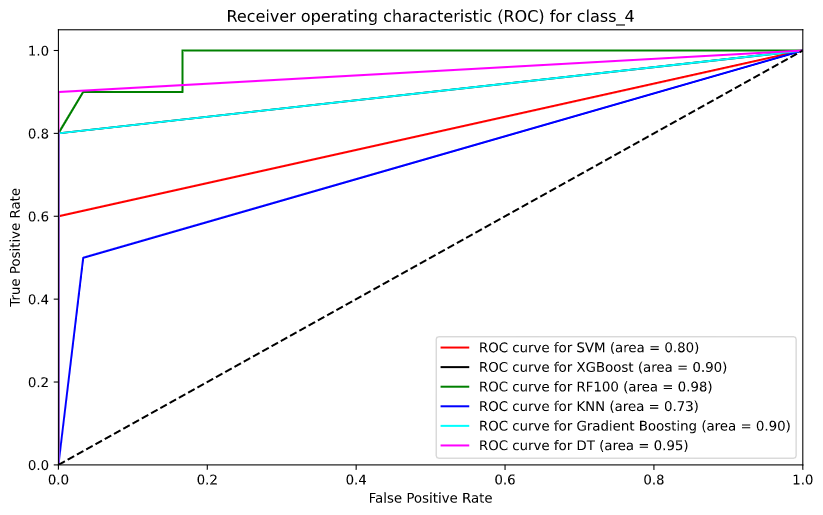
\includegraphics[scale=0.25]{fig/roc4.png}
    \caption{Receiver operating characteristic (ROC) - $class_4$}
    \label{fig:roc4}
    \end{subfigure}
    \caption{Receiver operating characteristic (ROC) para os classificadores apresentados.}
    \label{roc}
\end{figure}

Após isso comparamos os resultados das acurácias através de um \textit{radarplot} (Figura \ref{fig:radar}) e um \textit{barplot} (Figura \ref{fig:barplot}):

\begin{verbatim}
 #file: comparison.ipynb
 #Radarplot
 df_rplot = pd.DataFrame(dict(ac=[ac_xgb, ac_svm, ac_rf, ac_knn, ac_gb,
 ac_dt],
                             names_classif=['XGB','SVM', 'RF', 'KNN', 'GB',
                             'DT']))
 fig = px.line_polar(df_rplot, 
                     r='ac', 
                     theta='names_classif', 
                     line_close=True, 
                     title='Radarplot - Accuracy')
 fig.update_traces(fill='toself')
 fig.show()
 #Barplot
 fig = plt.figure(figsize=(10,4))
 ax = fig.add_axes([0,0,1,1])
 name_classifier=['XG Boost','SVM', 'Random Forest', 'KNN', 'Gradient
 Boost.', 'Decion Tree']
 ac=[ac_xgb, ac_svm, ac_rf, ac_knn, ac_gb, ac_dt]
 bar = ax.bar(name_class,ac, color=['black', 'red', 'green', 'blue', 'cyan',
 'magenta'])
 labels = name_classifier
 opacity = 0.4
 bar_width = 0.35
 for rect, label in zip(bar, labels):
     height = rect.get_height()
     plt.text(rect.get_x() + rect.get_width() / 2.0, height, label,
     ha='center', va='bottom')
 ax.set_ylabel('Accuracy')
 ax.set_title('Accuracy by Classifier')
 plt.show()
\end{verbatim}


\begin{figure}[H]
 \centering
 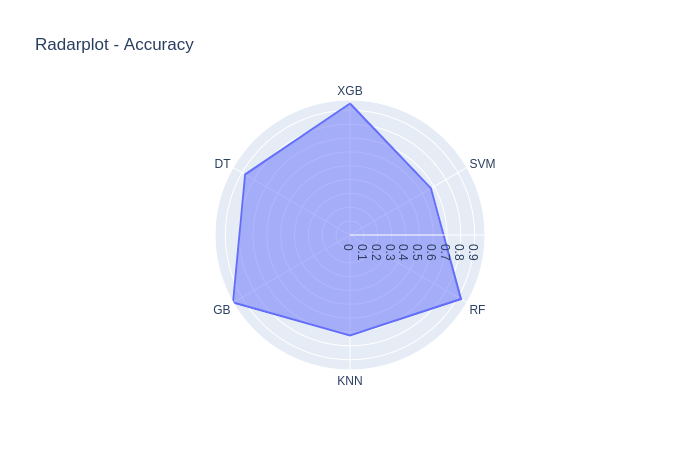
\includegraphics[scale=0.5]{fig/radarplot.png}
 % scatter.png: 619x604 px, 96dpi, 16.38x15.98 cm, bb=0 0 464 453
 \caption{Radarplot da acurácia dos métodos analisados.}
 \label{fig:radar}
\end{figure}

\begin{figure}[H]
 \centering
 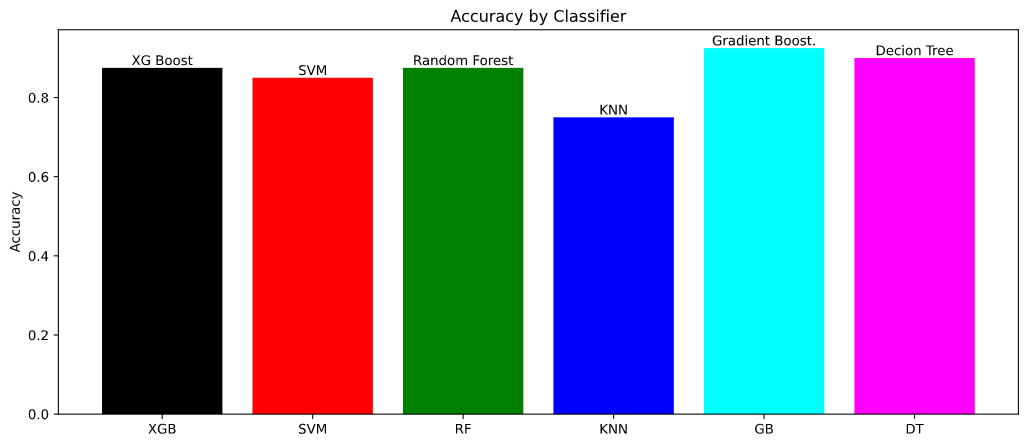
\includegraphics[scale=0.4]{fig/barplot.png}
 % scatter.png: 619x604 px, 96dpi, 16.38x15.98 cm, bb=0 0 464 453
 \caption{Barplot da acurácia dos métodos analisados.}
 \label{fig:barplot}
\end{figure}

A advertência em relação a análise está na queantidade da dados utilizados para a geração das métricas, como já apresentado acima, estes valores estão restritos ao dataset e observações utilizadas, portanto a existência de valores ótimos em relação a métrica está diretamente relacionado a isso para cada uma das classes. Análises com um maior número de observações é necessária para a confirmação dos resultados, visto que em algumas classes o desempenho é exímio, não apresentando nenhum erro, o que na prática é uma situação muito difícil de ocorrer em todos os exemplares de teste. Diante disso, a comparação dos métodos foi capaz de mostrar que para esse dataset e metodologia adotada o método Gradient Boosting obteve uma maior acurácia quando comparado com os demais métodos, por outro lado métodos baseados em árvores sobressaíram aos outros métodos como $k-NN$ e SVM. 

% ----------------------------------------------------------
% ELEMENTOS PÓS-TEXTUAIS
% ----------------------------------------------------------
\postextual

% ----------------------------------------------------------
% Referências bibliográficas
% ----------------------------------------------------------
\bibliography{refs}

% ----------------------------------------------------------
% Glossário
% ----------------------------------------------------------
%
% Há diversas soluções prontas para glossário em LaTeX. 
% Consulte o manual do abnTeX2 para obter sugestões.
%
%\glossary

% ----------------------------------------------------------
% Apêndices
% ----------------------------------------------------------

% ---
% Inicia os apêndices
% ---
%\begin{apendicesenv}

% ----------------------------------------------------------
%\chapter{AA}
% ----------------------------------------------------------


%\end{apendicesenv}
% ---

% ----------------------------------------------------------
% Anexos
% ----------------------------------------------------------
%\cftinserthook{toc}{AAA}
% ---
% Inicia os anexos
% ---
%\anexos
%\begin{anexosenv}

% ---
%\chapter{Cras non urna sed feugiat cum sociis natoque penatibus et magnis dis
%parturient montes nascetur ridiculus mus}
% ---

%\lipsum[31]

%\end{anexosenv}

% ----------------------------------------------------------
% Agradecimentos
% ----------------------------------------------------------

%\section*{Agradecimentos}
%Texto sucinto aprovado pelo periódico em que será publicado. Último 
%elemento pós-textual.

\end{document}
